\documentclass[12pt]{article}
\usepackage{amsmath}
\usepackage{graphicx}
\usepackage{hyperref}
\usepackage{natbib}
\usepackage{amsthm}
\usepackage{amssymb}
\usepackage{algorithm}
\usepackage{algpseudocode}
\usepackage{booktabs}
\usepackage{enumitem}
\usepackage{bm}
\usepackage{multirow}
\usepackage[margin=1in]{geometry}
\usepackage{tikz}
\usepackage{pgfplots}
\pgfplotsset{compat=1.17}
\usetikzlibrary{arrows.meta, positioning, calc, patterns, decorations.pathreplacing, backgrounds, fit, shapes.geometric, matrix}

\newcommand{\R}{\mathbb{R}}
\newcommand{\Z}{\mathbb{Z}}
\newcommand{\E}{\mathbb{E}}
\newcommand{\norm}[1]{\left\lVert #1 \right\rVert}
\newcommand{\argsort}{\mathrm{argsort}}
\newcommand{\rankop}{\mathrm{rank}}
\newcommand{\softmax}{\mathrm{softmax}}

\newtheorem{theorem}{Theorem}
\newtheorem{lemma}[theorem]{Lemma}
\newtheorem{corollary}[theorem]{Corollary}
\newtheorem{proposition}[theorem]{Proposition}
\newtheorem{definition}[theorem]{Definition}
\newtheorem{remark}{Remark}

\begin{document}

\title{ArrowFlow: Hierarchical Machine Learning\\in the Space of Permutations}
\author{Ozgur Yilmaz\footnote{ozguryilmaz@atu.edu.tr; \url{https://scholar.google.com/citations?user=AIJWYCAAAAAJ}} \\
\small Department of Artificial Intelligence\\
\small Adana Science and Technology University, Adana, Turkey}
\date{}
\maketitle

% ============================================================================
% ABSTRACT
% ============================================================================
\begin{abstract}
We introduce \textbf{ArrowFlow}, a machine learning architecture that operates entirely in the space of permutations. Its computational units are \emph{ranking filters}---learned orderings that compare inputs via Spearman's footrule distance and update through permutation-matrix accumulation, a non-gradient rule rooted in displacement evidence. Layers compose hierarchically: each layer's output ranking becomes the next layer's input, enabling deep ordinal representation learning without any floating-point parameters in the core computation.

An encoding pipeline (polynomial expansion, random projection, argsort) bridges real-valued data and the permutation world, while a multi-view ensemble---independent networks trained on diverse projections, combined by majority vote---compensates for information lost in the ordinal encoding. We connect the architecture to Arrow's impossibility theorem, showing that violations of social-choice fairness axioms (context dependence, specialization, symmetry breaking) serve as inductive biases for nonlinearity, sparsity, and stability.

Experiments span UCI tabular benchmarks, MNIST, gene expression cancer classification (TCGA), and preference data, all against GridSearchCV-tuned baselines. ArrowFlow beats all baselines on Iris (2.7\% vs.\ 3.3\%) and is competitive on most UCI datasets. On gene expression data, rank-based methods achieve \emph{perfect invariance} to monotone batch effects (stable at 2.5\% where SVM on raw values collapses to 82.6\%). On MNIST via PCA, ArrowFlow reaches 9.1\% error using only ordinal comparisons, with strong scaling as network width and depth increase. A single parameter---polynomial degree---acts as a master switch: degree 1 yields noise robustness (8--28\% less degradation), privacy preservation (+0.5pp cost), and missing-feature resilience; higher degrees trade these for improved clean accuracy.

ArrowFlow is not designed to surpass gradient-based methods. It is an existence proof that competitive classification is possible in a fundamentally different computational paradigm---one that elevates ordinal structure to a first-class citizen, with natural alignment to integer-only and neuromorphic hardware.

\medskip
\noindent\textbf{Code:} \url{https://github.com/yilmazozgur/arrowflow}
\end{abstract}

% ============================================================================
% 1. INTRODUCTION
% ============================================================================
\section{Introduction}
\label{sec:intro}

The dominant paradigm in modern machine learning represents data as real-valued tensors and learns transformations through gradient descent on differentiable, continuous parameter spaces. While extraordinarily successful, this paradigm has fundamental limitations when the underlying structure of data is \emph{ordinal} or \emph{relational} rather than metric. Consider classifying sequences by their ordering pattern: the sequence $[1, 2, 3, 4, 5]$ is ``ascending'' and $[5, 4, 3, 2, 1]$ is ``descending.'' The essential information is not the magnitude of elements but their \emph{relative ordering}---a combinatorial, not metric, property.

ArrowFlow is built on the premise that \textbf{the fundamental data structure in a neural network can be a sorted list, and the fundamental operation can be the edit distance between two such lists}. In this framework:

\begin{itemize}[leftmargin=2em]
  \item \textbf{Data points} are ordered sequences of tokens (permutations of a vocabulary).
  \item \textbf{Learned filters} are also permutations of the same vocabulary.
  \item \textbf{Similarity} is measured by Spearman's footrule distance---the sum of absolute positional displacements between two orderings \citep{diaconis1977footrule}.
  \item \textbf{Learning} proceeds by re-ordering filter elements based on accumulated displacement evidence, rather than by adjusting floating-point weights.
\end{itemize}

This architecture draws from a productive tension in social choice theory. Arrow's impossibility theorem \citep{arrow1951social} demonstrates that any aggregator of individual rankings must violate at least one fairness axiom (Pareto efficiency, independence of irrelevant alternatives, non-dictatorship) on some preference profiles. In learning, we \emph{exploit} these violations as inductive biases: context dependence (IIA violations) yields nonlinearity; specialization (ND violations) yields sparsity and winner-take-all dynamics; partial monotonicity (Pareto-like behavior) stabilizes training. The name ``ArrowFlow'' reflects both this connection to Arrow's theorem and the flow of ordering information through the network layers.

\paragraph{What ArrowFlow is---and is not.}
ArrowFlow is not designed to be the most accurate or fastest classifier. It is a \emph{fundamentally different computational paradigm}: a hierarchical, filter-based machine learning system that operates entirely in the space of permutations. The contribution is the paradigm itself---showing that competitive classification is achievable without any floating-point parameters in the core computation, and that ordinal architectures possess structural advantages (noise robustness, privacy preservation, graceful handling of missing data) that are absent from conventional methods.

\paragraph{Contributions.}
\begin{enumerate}[leftmargin=2em]
  \item A formal definition of the \emph{ranking layer} with edit-distance motions, permutation-matrix accumulation, and hierarchical rank aggregation (Section~\ref{sec:ranking-layer}).
  \item The multi-view ensemble architecture with diverse projection strategies that addresses the argsort encoding bottleneck and achieves competitive accuracy (Sections~\ref{sec:encoding}--\ref{sec:ensemble}).
  \item An Arrow-theoretic interpretation of layer expressivity, connecting fairness-axiom violations to inductive biases for nonlinearity, sparsity, and stability (Section~\ref{sec:arrow}).
  \item Formal theoretical analysis: an argsort stability theorem with Gaussian tail bound (explaining noise robustness), an information-capacity theorem ($\log_2(d!)$ bits via permutation cones), a polynomial noise amplification result (explaining the accuracy--robustness trade-off), a consistency proof for the accumulation learning rule, an ensemble error bound, and a social choice theory subsection that proves filter learning is maximum-likelihood estimation under the Mallows model, derives two-sided adversarial manipulability bounds from the Gibbard--Satterthwaite theorem, and quantifies IIA-violation as a measure of nonlinear expressivity (Section~\ref{sec:theory}).
  \item Comprehensive experiments across UCI tabular benchmarks, MNIST (via PCA, isolating the sort-layer classifier), gene expression cancer classification (TCGA), and the Sushi preference dataset. These reveal a unique robustness profile governed by the polynomial degree parameter, perfect batch-effect invariance under monotone distribution shifts, and architecture scaling that has not plateaued at 1024 filters (Sections~\ref{sec:experiments}--\ref{sec:utility}).
  \item A quantitative energy analysis showing that ArrowFlow's integer-only arithmetic is 15$\times$ cheaper per layer than equivalent FP32 MLP layers, with natural alignment to neuromorphic hardware and sorting-network implementations (Section~\ref{sec:energy}).
\end{enumerate}

\paragraph{Note.} This is an extended technical report presenting the full theory, experiments, and discussion for ArrowFlow. A shorter version is in preparation for submission to JMLR or Neurocomputing.

% --- Figure 1: ArrowFlow Pipeline (Hero Figure) ---
\begin{figure}[t]
\centering
\resizebox{\textwidth}{!}{%
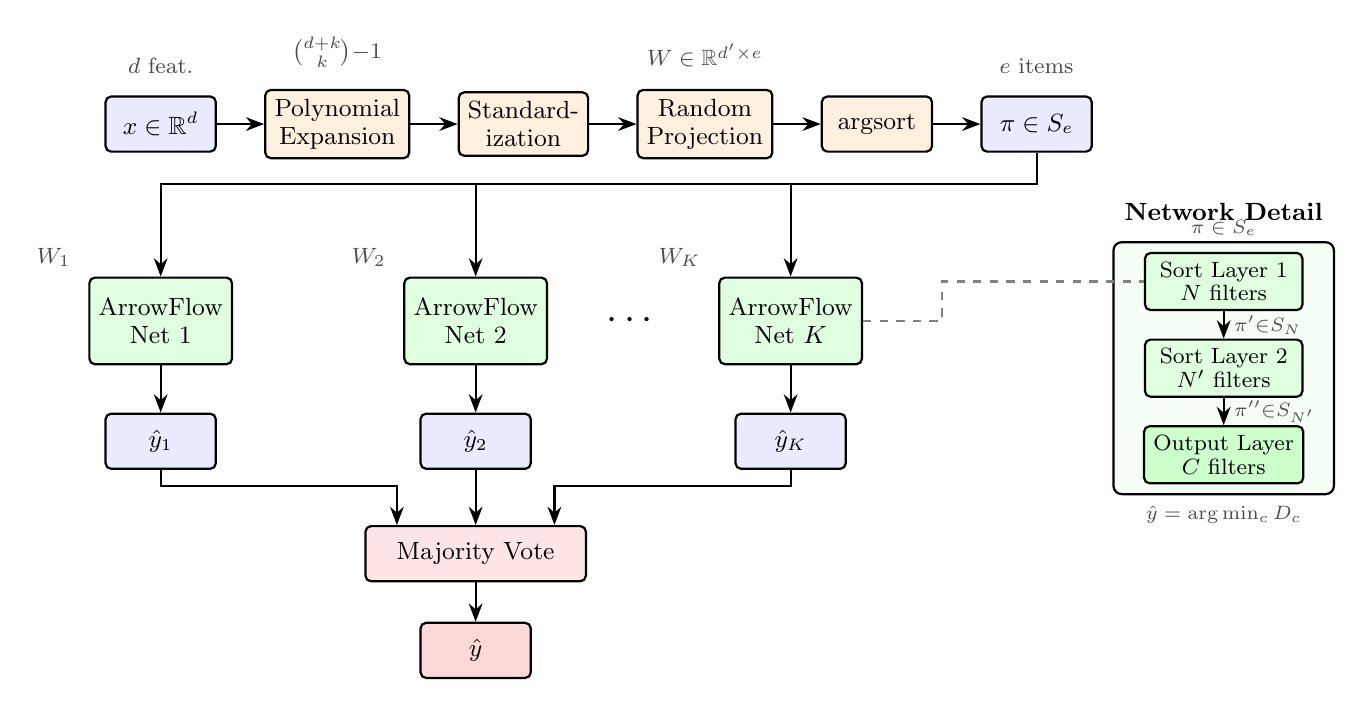
\begin{tikzpicture}[
    >=Stealth,
    box/.style={draw, rounded corners=2pt, minimum height=0.7cm, minimum width=1.4cm,
                font=\small, align=center, thick},
    databox/.style={box, fill=blue!8},
    procbox/.style={box, fill=orange!12},
    sortbox/.style={box, fill=green!12},
    votebox/.style={box, fill=red!10},
    arr/.style={->, thick},
    lbl/.style={font=\footnotesize, text=black!70},
]
% === Encoding pipeline (top row) ===
\node[databox] (input) at (0,0) {$x \in \R^d$};
\node[procbox, right=0.6 of input] (poly) {Polynomial\\[-1pt]Expansion};
\node[procbox, right=0.6 of poly] (std) {Standard-\\[-1pt]ization};
\node[procbox, right=0.6 of std] (proj) {Random\\[-1pt]Projection};
\node[procbox, right=0.6 of proj] (args) {$\argsort$};
\node[databox, right=0.6 of args] (perm) {$\pi \in S_e$};
\draw[arr] (input) -- (poly);
\draw[arr] (poly) -- (std);
\draw[arr] (std) -- (proj);
\draw[arr] (proj) -- (args);
\draw[arr] (args) -- (perm);
\node[lbl, above=0.15 of input] {$d$ feat.};
\node[lbl, above=0.15 of poly] {$\binom{d+k}{k}{-}1$};
\node[lbl, above=0.15 of proj] {$W \in \R^{d'\times e}$};
\node[lbl, above=0.15 of perm] {$e$ items};
% === Multi-view branching (3 networks) ===
\node[sortbox, minimum height=1.1cm] (net1) at (0, -2.5) {ArrowFlow\\[-1pt]Net 1};
\node[sortbox, minimum height=1.1cm] (net2) at (4, -2.5) {ArrowFlow\\[-1pt]Net 2};
\node[sortbox, minimum height=1.1cm] (netK) at (8, -2.5) {ArrowFlow\\[-1pt]Net $K$};
\node at ($(net2)!0.5!(netK)$) {\Large$\cdots$};
\node[lbl, above left=0.0 and 0.1 of net1] {$W_1$};
\node[lbl, above left=0.0 and 0.1 of net2] {$W_2$};
\node[lbl, above left=0.0 and 0.1 of netK] {$W_K$};
% Branching arrows from perm
\draw[arr] (perm.south) -- ++(0,-0.4) -| (net1.north);
\draw[arr] (perm.south) -- ++(0,-0.4) -| (net2.north);
\draw[arr] (perm.south) -- ++(0,-0.4) -| (netK.north);
% === Predictions ===
\node[databox, below=0.6 of net1] (pred1) {$\hat{y}_1$};
\node[databox, below=0.6 of net2] (pred2) {$\hat{y}_2$};
\node[databox, below=0.6 of netK] (predK) {$\hat{y}_K$};
\draw[arr] (net1) -- (pred1);
\draw[arr] (net2) -- (pred2);
\draw[arr] (netK) -- (predK);
% === Majority vote ===
\node[votebox, below=0.7 of pred2, minimum width=2.8cm] (vote) {Majority Vote};
\draw[arr] (pred1.south) -- ++(0,-0.2) -| (vote.160);
\draw[arr] (pred2) -- (vote);
\draw[arr] (predK.south) -- ++(0,-0.2) -| (vote.20);
\node[databox, below=0.5 of vote, fill=red!15] (final) {$\hat{y}$};
\draw[arr] (vote) -- (final);
% === Network detail inset (far right, well separated) ===
\begin{scope}[shift={(13.5,-1.5)}]
\node[font=\small\bfseries, anchor=south] at (0,0.15) {Network Detail};
\draw[thick, rounded corners=3pt, fill=green!4] (-1.4,-3.2) rectangle (1.4,0);
\node[sortbox, minimum width=2.0cm, font=\footnotesize] (L1) at (0,-0.5) {Sort Layer 1\\[-1pt]$N$ filters};
\node[sortbox, minimum width=2.0cm, font=\footnotesize] (L2) at (0,-1.6) {Sort Layer 2\\[-1pt]$N'$ filters};
\node[sortbox, minimum width=2.0cm, fill=green!20, font=\footnotesize] (Lout) at (0,-2.7) {Output Layer\\[-1pt]$C$ filters};
\draw[arr] (L1) -- node[lbl, right, font=\scriptsize] {$\pi'{\in}S_N$} (L2);
\draw[arr] (L2) -- node[lbl, right, font=\scriptsize] {$\pi''{\in}S_{N'}$} (Lout);
\node[lbl, above=0.08 of L1, font=\scriptsize] {$\pi \in S_e$};
\node[lbl, below=0.15 of Lout, font=\scriptsize] {$\hat{y} = \arg\min_c D_c$};
\end{scope}
% Dashed connector from network box to inset
\draw[dashed, gray, thick] (netK.east) -- ++(1.0,0) |- (L1.west);
\end{tikzpicture}%
}
\caption{\textbf{ArrowFlow pipeline.} Real-valued input $x$ is encoded via polynomial expansion, standardization, random projection, and argsort. $K$ independent networks receive different projections $W_k$. Each network (detail, right) is a stack of sort layers computing Spearman's footrule distance to learned filters. Predictions are combined by majority vote.}
\label{fig:pipeline}
\end{figure}


% ============================================================================
% 2. RELATED WORK
% ============================================================================
\section{Related Work}
\label{sec:related}

ArrowFlow sits at the intersection of several research traditions: neuroscience-inspired rank-order coding, differentiable sorting, permutation distance metrics, non-gradient learning, social choice theory, random projections, and ensemble methods. We survey each in turn, positioning ArrowFlow's contributions relative to prior work.

\subsection{Rank Order Coding}
Rank Order Coding (ROC) encodes stimulus strength via the \emph{order} of neural spikes rather than absolute firing rates, highlighting order as an information carrier \citep{thorpe1998rapid, gautrais1998rate}. This biological principle---that relative ordering is more robust and efficient than precise magnitude encoding---motivates ArrowFlow's core design. The approach has shown promise in image recognition, where relative pixel intensities can be more informative than precise values under varying conditions \citep{jost2002rank, bonilla2022analyzing}. ArrowFlow generalizes ROC from a fixed encoding scheme to a \emph{learnable hierarchical transformation} of orderings across layers.

\subsection{Differentiable Sorting and Sinkhorn Networks}
Recent work has made sorting operations differentiable for end-to-end learning. NeuralSort \citep{grover2019neuralsort} and SoftSort \citep{prillo2020softsort} provide continuous relaxations of argsort. Blondel et al.\ \citep{blondel2020fast} introduced fast differentiable sorting via optimal transport. Gumbel-Sinkhorn networks \citep{mena2018gumbelsinkhorn} learn latent permutations through doubly stochastic matrices, leveraging the classical Sinkhorn normalization \citep{sinkhorn1967diagonal}. These approaches treat order as a soft surrogate for continuous scores---they relax permutations everywhere to enable gradient flow. ArrowFlow takes the opposite approach: it \textbf{operates directly on discrete permutations} and replaces gradient descent with permutation-matrix-based updates. Differentiability is needed only at the boundaries between rank and tensor layers, not within the ranking computation itself.

\subsection{Permutation Distance Metrics}
Kendall \citep{kendall1938} introduced the tau rank correlation coefficient, counting pairwise disagreements. Diaconis and Graham \citep{diaconis1977footrule} established Spearman's footrule as a closely related metric, proving that footrule and Kendall tau distance are within a constant factor. ArrowFlow uses Spearman's footrule ($\ell_1$ norm of positional displacements) as its core distance. Fagin et al.\ \citep{fagin2003topk} extended these metrics to partial rankings, relevant to ArrowFlow's handling of receptive fields and variable-length inputs.

\subsection{Non-Gradient Learning}
ArrowFlow's sort layers do not use gradient descent. The permutation-matrix accumulation rule connects to Kohonen's Self-Organizing Maps \citep{kohonen1990self}, which learn via competitive learning---the closest prototype is updated to become more similar to the input. The key difference is that ArrowFlow prototypes are permutations updated by re-ordering, not real-valued vectors updated by subtraction. This competitive dynamic also relates to Grossberg's Adaptive Resonance Theory \citep{grossberg1987competitive}, where winner-take-all prototypes are updated by matching and accumulation. Pointer Networks \citep{vinyals2015pointernetworks} and the ``Order Matters'' framework \citep{vinyals2015order} demonstrated that input and output ordering significantly impacts sequence-to-sequence performance, motivating architectures that treat ordering as a learnable structure. More recently, Hinton's Forward-Forward algorithm \citep{hinton2022forward} and Target Propagation \citep{lee2015difference} have revived interest in alternatives to backpropagation. ArrowFlow contributes to this line by demonstrating that competitive, displacement-based learning can work in discrete permutation spaces.

\subsection{Social Choice Theory and Rank Aggregation}
Arrow's impossibility theorem \citep{arrow1951social} demonstrates unavoidable trade-offs in rank aggregation---no mechanism aggregating three or more alternatives can simultaneously satisfy Pareto efficiency, independence of irrelevant alternatives, and non-dictatorship. Rank aggregation has been extensively studied in information retrieval, where Dwork et al.\ \citep{dwork2001rank} proposed combining ranked results from multiple search engines using median-based methods on Kendall tau distance. The Mallows model \citep{mallows1957nonnull} provides a probabilistic framework for permutations centered on a modal ranking, parameterized by a dispersion parameter. Conitzer and Sandholm \citep{conitzer2005voting} showed that common voting rules (Borda, Kemeny) correspond to maximum likelihood estimation under different noise models over permutations, providing a statistical-learning interpretation of the social-choice concepts that ArrowFlow operationalizes. Rank-Ordered Autoencoders \citep{bertens2016rank} use rank-preserving embeddings and sparsity constraints. ArrowFlow generalizes from \emph{preserving} rank to \emph{transforming} rank across layers, and uniquely reinterprets Arrow's fairness-axiom violations as inductive biases for nonlinearity, sparsity, and stability.

\subsection{Random Projections and Dimensionality Reduction}
ArrowFlow's encoding pipeline relies on random projection to map data into a space where argsort produces informative permutations. The Johnson-Lindenstrauss lemma \citep{johnson1984extensions} guarantees that random projections approximately preserve pairwise distances. Achlioptas \citep{achlioptas2003database} showed that even very sparse random matrices suffice for this purpose. Arriaga and Vempala \citep{arriaga2006algorithmic} proved that random projections preserve margin-based learnability, directly justifying ArrowFlow's pipeline of random projection followed by classification. Cannings and Samworth \citep{cannings2017random} proposed random-projection ensemble classification, combining classifiers trained on different random projections via data-driven voting---ArrowFlow's multi-view ensemble is a permutation-space instance of exactly this framework.

\subsection{Ensemble Methods and Multi-View Learning}
ArrowFlow's multi-view ensemble draws on classical ensemble theory. Breiman's bagging \citep{breiman1996bagging} established variance reduction through bootstrap aggregation. Schapire \citep{schapire1990strength} proved that any weak learner can be boosted to arbitrary accuracy, providing theoretical grounding for why ArrowFlow's individual views, even if weak, combine into a strong ensemble. Dietterich \citep{dietterich2000ensemble} showed that ensemble diversity is as important as individual accuracy. Condorcet's jury theorem provides the theoretical foundation: if each voter has error rate $p < 0.5$ and errors are independent, the majority-vote error decreases exponentially with the number of voters. ArrowFlow maximizes the independence condition by using diverse projection strategies---each view sees a different ordinal representation of the same data. This connects to the multi-view learning framework of Xu et al.\ \citep{xu2013survey}, where complementary ``views'' are fused for improved prediction.

\subsection{Robustness Through Discretization}
A distinctive finding of ArrowFlow is that the argsort discretization provides measurable noise robustness when polynomial expansion is absent. This connects to a broader literature on discretization for robustness. Quantization-aware training \citep{jacob2018quantization} shows that reduced-precision representations can improve robustness. The VQ-VAE \citep{oord2017neural} demonstrated that discretizing latent representations via vector quantization improves generalization and avoids posterior collapse---ArrowFlow's argsort is an extreme form of discretization that converts continuous features to combinatorial objects. More directly, the rank transform \citep{conover1981rank} has long been used in nonparametric statistics precisely because it is immune to monotone transformations and outliers. ArrowFlow's encoding pipeline makes this classical statistical insight into an architectural principle.

\subsection{Learning to Rank}
ArrowFlow also connects to the learning-to-rank literature in information retrieval, where the goal is to learn a function that orders items by relevance. RankNet \citep{burges2005learning} uses gradient descent on pairwise ranking losses; LambdaMART \citep{burges2010ranknet} combines boosted trees with ranking-specific objectives. These methods learn continuous scoring functions whose \emph{output} is a ranking. ArrowFlow inverts this relationship: both the \emph{input} and the \emph{learned parameters} are rankings, and learning operates by re-ordering filters rather than adjusting scores. This makes ArrowFlow more akin to a nearest-neighbor method in permutation metric space, enhanced with hierarchical learned embeddings.


% ============================================================================
% 3. THE RANKING LAYER
% ============================================================================
\section{The Ranking Layer}
\label{sec:ranking-layer}

The ranking layer is the fundamental computational unit of ArrowFlow. It operates in the space of orderings rather than numeric activations. Each layer transforms an input ranking into a new ranking representation by comparing it to a bank of learned \emph{ranking filters}.

\subsection{Notation}
Let $\mathcal{V} = \{1, \dots, V\}$ denote a vocabulary of tokens. A ranking is a permutation $\pi \in S_V$, where $\pi(i)$ gives the position of token $i$. We write $\argsort(y)$ for the permutation induced by sorting scores $y \in \R^V$ in descending order. For a filter $r$ and input $x$, $\rankop(r, x[p])$ denotes the position of element $x[p]$ in the filter's ordering.

\subsection{Ranking Filters and Edit-Distance Motions}
A ranking layer $F^{\mathrm{rank}}$ contains $N$ ranking filters $\{r_j\}_{j=1}^N$, each storing a learned local ordering over the vocabulary. Given an input ranking $\pi_x$, the layer computes an \emph{edit-motion} vector $m_j \in \Z^\ell$ for each filter:
\begin{equation}
m_j[p] = \rankop(r_j, \pi_x[p]) - p, \quad p = 1, \dots, \ell.
\label{eq:motion}
\end{equation}
The motion $m_j[p]$ measures how many positions element $\pi_x[p]$ must move to reach its position in filter $r_j$. This is a signed displacement---positive means the element should move toward the end, negative toward the front.

A distance is computed via the $\ell_q$ norm:
\begin{equation}
D_j = \norm{m_j}_q, \quad q \in \{0, 1, 2\}.
\label{eq:distance}
\end{equation}
With $q = 1$, this is Spearman's footrule distance \citep{diaconis1977footrule}: the total positional displacement between the input and the filter.

\paragraph{Missing data and receptive fields.}
If $\pi_x$ omits items present in $r_j$, the missing items are treated as displaced to the end, incurring a deletion penalty. If $r_j$ has a restricted receptive field (subset of items), the average motion is subtracted to promote translation invariance---analogous to zero-centering in convolutional layers.

\subsection{Forward Pass: From Distances to Output Ranking}
The layer aggregates $N$ filter responses into a new ranking. The simplest and most effective aggregation is:
\begin{equation}
\pi' = \argsort(-D_1, -D_2, \dots, -D_N),
\end{equation}
which ranks filters from closest (most similar) to farthest. The output $\pi'$ is a permutation of filter indices---a new sorted list in a vocabulary of size $N$---and becomes the input to the next layer.

This is a discrete analogue of convolution: filters ``slide'' over the input ordering, measure similarity via edit distance, and the resulting ordering defines the next representation.

% --- Figure 2: Ranking Layer Forward Pass ---
\begin{figure}[t]
\centering
\resizebox{\textwidth}{!}{%
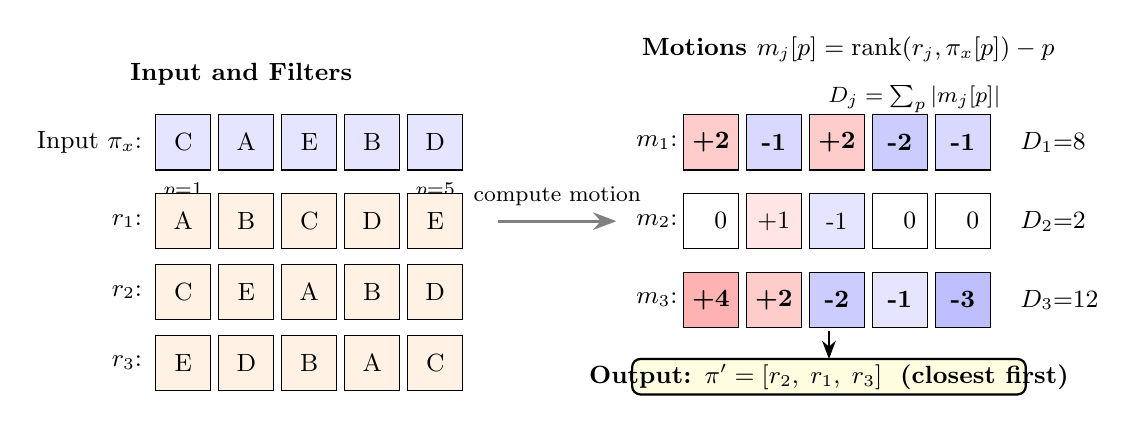
\begin{tikzpicture}[
    >=Stealth,
    arr/.style={->, thick},
    lbl/.style={font=\small},
    cell/.style={draw, minimum width=0.7cm, minimum height=0.7cm, font=\small, inner sep=0pt},
    hcell/.style={cell, fill=blue!10},
    fcell/.style={cell, fill=orange!10},
    mcell/.style={cell, fill=green!10},
]
% === LEFT HALF: Input + Filters ===
% Title
\node[font=\small\bfseries, anchor=south west] at (0.5, 1.8) {Input and Filters};
%
\node[lbl, anchor=east] at (0.9, 1.2) {Input $\pi_x$:};
\foreach \i/\v in {1/C, 2/A, 3/E, 4/B, 5/D} {
    \node[hcell] (in\i) at (0.5+\i*0.8, 1.2) {\v};
}
\node[lbl, below=0.04 of in1, font=\scriptsize] {$p{=}1$};
\node[lbl, below=0.04 of in5, font=\scriptsize] {$p{=}5$};
%
\node[lbl, anchor=east] at (0.9, 0.2) {$r_1$:};
\foreach \i/\v in {1/A, 2/B, 3/C, 4/D, 5/E} {
    \node[fcell] (f1\i) at (0.5+\i*0.8, 0.2) {\v};
}
\node[lbl, anchor=east] at (0.9, -0.7) {$r_2$:};
\foreach \i/\v in {1/C, 2/E, 3/A, 4/B, 5/D} {
    \node[fcell] (f2\i) at (0.5+\i*0.8, -0.7) {\v};
}
\node[lbl, anchor=east] at (0.9, -1.6) {$r_3$:};
\foreach \i/\v in {1/E, 2/D, 3/B, 4/A, 5/C} {
    \node[fcell] (f3\i) at (0.5+\i*0.8, -1.6) {\v};
}
% === Arrow between halves (above the rows, no overlap) ===
\draw[arr, gray, very thick] (5.3, 0.2) -- (6.8, 0.2);
\node[font=\footnotesize, black, above=2pt] at (6.05, 0.2) {compute motion};
% === RIGHT HALF: Motions ===
% Title
\node[font=\small\bfseries, anchor=south west] at (7.0, 2.1) {Motions $m_j[p] = \mathrm{rank}(r_j, \pi_x[p]) - p$};
%
\node[lbl, anchor=east] at (7.7, 1.2) {$m_1$:};
\foreach \i/\v/\c in {1/{+2}/red!20, 2/{-1}/blue!15, 3/{+2}/red!20, 4/{-2}/blue!20, 5/{-1}/blue!15} {
    \node[mcell, fill=\c, font=\small\bfseries] (m1\i) at (7.2+\i*0.8, 1.2) {\v};
}
\node[lbl, right=0.25 of m15] {$D_1{=}8$};
%
\node[lbl, anchor=east] at (7.7, 0.2) {$m_2$:};
\foreach \i/\v/\c in {1/{\phantom{+}0}/white, 2/{+1}/red!10, 3/{-1}/blue!10, 4/{\phantom{+}0}/white, 5/{\phantom{+}0}/white} {
    \node[mcell, fill=\c, font=\small] (m2\i) at (7.2+\i*0.8, 0.2) {\v};
}
\node[lbl, right=0.25 of m25] {$D_2{=}2$};
%
\node[lbl, anchor=east] at (7.7, -0.8) {$m_3$:};
\foreach \i/\v/\c in {1/{+4}/red!30, 2/{+2}/red!20, 3/{-2}/blue!20, 4/{-1}/blue!10, 5/{-3}/blue!25} {
    \node[mcell, fill=\c, font=\small\bfseries] (m3\i) at (7.2+\i*0.8, -0.8) {\v};
}
\node[lbl, right=0.25 of m35] {$D_3{=}12$};
% Formula note (below title, right-aligned)
\node[font=\footnotesize, anchor=east] at (11.8, 1.75) {$D_j = \sum_p |m_j[p]|$};
% === Output ranking ===
\draw[thick, rounded corners=3pt, fill=yellow!12] (7.0,-2.0) rectangle (12.0,-1.55);
\node[font=\small\bfseries] at (9.5,-1.78) {Output: $\pi' = [r_2,\; r_1,\; r_3]$ \;\small(closest first)};
\draw[arr, thick] (9.5, -1.2) -- (9.5, -1.55);
\end{tikzpicture}%
}
\caption{\textbf{Ranking layer forward pass.} Input $\pi_x = [C, A, E, B, D]$ is compared to three filters. The motion $m_j[p] = \mathrm{rank}(r_j, \pi_x[p]) - p$ measures signed displacement (red = forward, blue = backward). The footrule distance $D_j = \sum |m_j[p]|$ totals the displacements. Filters are ranked by proximity: $r_2$ (distance 2) is closest. The output $\pi'$ becomes the input to the next layer.}
\label{fig:forward-pass}
\end{figure}

\subsection{Backward Pass: Motion as Discrete Gradient}

The key insight is that the motion vector $m_j$ from Eq.~\eqref{eq:motion} plays the role of a gradient in continuous optimization---it tells us \emph{how to move each element} to reduce distance.

\begin{proposition}[Motion as Discrete Gradient]
\label{prop:motion-gradient}
Given $d_F(\pi_x, r_j) = \sum_{p=1}^\ell |m_j[p]|$, the displacement $m_j[p]$ from Eq.~\eqref{eq:motion} is the unique per-position minimizer---the shift that zeroes item~$\pi_x[p]$'s footrule contribution:
for each~$p$,
\[
m_j[p] = \arg\min_{\delta \in \Z}\; \big|\rankop(r_j,\, \pi_x[p]) - (p + \delta)\big|.
\]
\end{proposition}

The motion vector thus points each item directly toward its target position in the filter, making it the discrete analogue of a loss gradient. The update signal comes from the motion between the input ordering and the correct-class filter. No calculus is involved.

\subsection{Permutation-Matrix Accumulation}
\label{sec:perm-accum}

Each filter $r_j$ maintains an accumulator $A_j \in \R^{V \times V}$ (initialized to identity) that integrates displacement votes across training examples. Given input $\pi_x$, the \emph{vote matrix} $\Phi(\pi_x, r_j) \in \{0,1\}^{V \times V}$ records where each item appears in the input:
\begin{definition}[Vote Matrix]
\label{def:vote-matrix}
Each item $v$ in the vocabulary votes for its position in the input $\pi_x$:
\[
\Phi(\pi_x, r_j)[v,\, k] = \begin{cases} 1 & \text{if } k = \rankop(\pi_x, v), \\ 0 & \text{otherwise,} \end{cases}
\]
where $\rankop(\pi_x, v)$ denotes the position of item $v$ in the input ordering $\pi_x$.
Each row of $\Phi$ has exactly one nonzero entry: item $v$ votes for the position that the training data places it at.
\end{definition}

Equivalently, for each filter position $p$, the backward motion $m_j^{\mathrm{bwd}}[p] = \rankop(\pi_x, r_j[p]) - p$ measures where filter item $r_j[p]$ appears in the input, and the vote places $r_j[p]$ at position $p + m_j^{\mathrm{bwd}}[p]$. Note that this backward motion is the negative of the forward motion from Eq.~\eqref{eq:motion}: the forward motion measures displacement \emph{from input to filter}, while the backward motion measures displacement \emph{from filter to input}, providing the update direction.

The accumulator is updated additively:
\begin{equation}
\label{eq:accum-update}
A_j \leftarrow A_j + \Phi(\pi_x, r_j).
\end{equation}
After $T$ updates, $A_j[v, k]$ counts the total evidence that item $v$ belongs at position $k$. The filter's ordering is recomputed via weighted index averaging:
\begin{equation}
\label{eq:accum-reorder}
\hat{\imath}(v) = \frac{\sum_k k \cdot A_j[v, k]}{\sum_k A_j[v, k]}, \qquad
r_j \leftarrow \argsort\big(\{\hat{\imath}(v)\}_{v \in \mathcal{V}}\big).
\end{equation}
This acts as a proximal step on the permutation manifold: accumulate displacement evidence, then project to the nearest ordering consistent with the aggregate evidence. The accumulator smooths individual motions and provides a form of momentum.

\begin{remark}
The learning rule has no learning rate in the continuous sense. Instead, the accumulator's history provides natural damping: recent motions contribute proportionally to the total accumulated evidence. An explicit learning rate $\eta$ can optionally scale the vote matrix $\Phi$ to control update speed.
\end{remark}

% --- Figure 3: Permutation-Matrix Accumulation ---
\begin{figure}[t]
\centering
\resizebox{0.95\textwidth}{!}{%
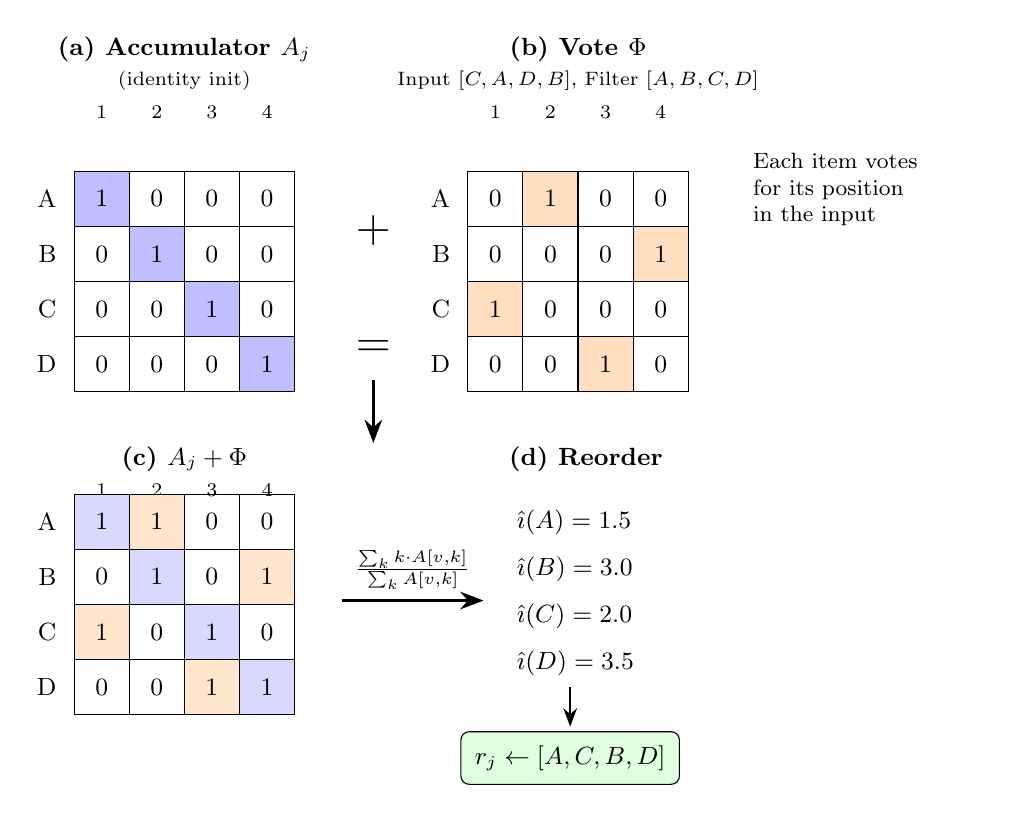
\begin{tikzpicture}[
    >=Stealth,
    arr/.style={->, thick},
    lbl/.style={font=\small},
    cell/.style={draw, minimum width=0.7cm, minimum height=0.7cm, font=\small, inner sep=0pt},
]
% ============================================================
% ROW 1:  (a) Accumulator   +   (b) Vote matrix
% ============================================================
% --- (a) title ---
\node[font=\small\bfseries] at (1.4, 3.7) {(a) Accumulator $A_j$};
\node[font=\scriptsize] at (1.4, 3.3) {(identity init)};
% column headers
\node[lbl, font=\scriptsize] at (0.35, 2.9) {1};
\node[lbl, font=\scriptsize] at (1.05, 2.9) {2};
\node[lbl, font=\scriptsize] at (1.75, 2.9) {3};
\node[lbl, font=\scriptsize] at (2.45, 2.9) {4};
% matrix
\foreach \r/\item in {1/A, 2/B, 3/C, 4/D} {
    \node[lbl, anchor=east] at (-0.1, 2.5-\r*0.7) {\item};
    \foreach \c in {1,2,3,4} {
        \pgfmathtruncatemacro{\val}{\r==\c ? 1 : 0}
        \pgfmathtruncatemacro{\shade}{\r==\c ? 25 : 0}
        \node[cell, fill=blue!\shade] at (-0.35+\c*0.7, 2.5-\r*0.7) {\val};
    }
}
% --- Plus sign (between matrices) ---
\node[font=\LARGE\bfseries] at (3.8, 1.4) {$+$};
% --- (b) title ---
\node[font=\small\bfseries] at (6.4, 3.7) {(b) Vote $\Phi$};
\node[font=\scriptsize] at (6.4, 3.3) {Input $[C,A,D,B]$, Filter $[A,B,C,D]$};
% column headers
\node[lbl, font=\scriptsize] at (5.35, 2.9) {1};
\node[lbl, font=\scriptsize] at (6.05, 2.9) {2};
\node[lbl, font=\scriptsize] at (6.75, 2.9) {3};
\node[lbl, font=\scriptsize] at (7.45, 2.9) {4};
% matrix
\foreach \r/\item/\votecol in {1/A/2, 2/B/4, 3/C/1, 4/D/3} {
    \node[lbl, anchor=east] at (4.9, 2.5-\r*0.7) {\item};
    \foreach \c in {1,2,3,4} {
        \pgfmathtruncatemacro{\val}{\c==\votecol ? 1 : 0}
        \pgfmathtruncatemacro{\shade}{\c==\votecol ? 25 : 0}
        \node[cell, fill=orange!\shade] at (4.65+\c*0.7, 2.5-\r*0.7) {\val};
    }
}
% --- Explanation (far right) ---
\node[lbl, text width=2.8cm, align=left, anchor=north west, font=\footnotesize] at (8.5, 2.5) {Each item votes\\for its position\\in the input};
% ============================================================
% Equals sign + down arrow
% ============================================================
\node[font=\LARGE\bfseries] at (3.8, -0.1) {$=$};
\draw[arr, very thick] (3.8, -0.5) -- (3.8, -1.3);
% ============================================================
% ROW 2:  (c) Updated accumulator    (d) Reorder
% ============================================================
% --- (c) title ---
\node[font=\small\bfseries] at (1.4, -1.5) {(c) $A_j + \Phi$};
% column headers
\node[lbl, font=\scriptsize] at (0.35, -1.9) {1};
\node[lbl, font=\scriptsize] at (1.05, -1.9) {2};
\node[lbl, font=\scriptsize] at (1.75, -1.9) {3};
\node[lbl, font=\scriptsize] at (2.45, -1.9) {4};
% matrix cells (identity + vote: A votes pos 2, B votes pos 4, C votes pos 1, D votes pos 3)
\node[lbl, anchor=east] at (-0.1, -2.3) {A};
\node[cell, fill=blue!15] at (0.35, -2.3) {1};
\node[cell, fill=orange!20] at (1.05, -2.3) {1};
\node[cell] at (1.75, -2.3) {0};
\node[cell] at (2.45, -2.3) {0};
%
\node[lbl, anchor=east] at (-0.1, -3.0) {B};
\node[cell] at (0.35, -3.0) {0};
\node[cell, fill=blue!15] at (1.05, -3.0) {1};
\node[cell] at (1.75, -3.0) {0};
\node[cell, fill=orange!20] at (2.45, -3.0) {1};
%
\node[lbl, anchor=east] at (-0.1, -3.7) {C};
\node[cell, fill=orange!20] at (0.35, -3.7) {1};
\node[cell] at (1.05, -3.7) {0};
\node[cell, fill=blue!15] at (1.75, -3.7) {1};
\node[cell] at (2.45, -3.7) {0};
%
\node[lbl, anchor=east] at (-0.1, -4.4) {D};
\node[cell] at (0.35, -4.4) {0};
\node[cell] at (1.05, -4.4) {0};
\node[cell, fill=orange!20] at (1.75, -4.4) {1};
\node[cell, fill=blue!15] at (2.45, -4.4) {1};
% --- Arrow from (c) to (d) ---
\draw[arr, very thick] (3.4, -3.3) -- node[above, font=\footnotesize] {$\frac{\sum_k k \cdot A[v,k]}{\sum_k A[v,k]}$} (5.2, -3.3);
% --- (d) title ---
\node[font=\small\bfseries] at (6.5, -1.5) {(d) Reorder};
% weighted averages
\node[lbl, anchor=west] at (5.5, -2.3) {$\hat{\imath}(A) = 1.5$};
\node[lbl, anchor=west] at (5.5, -2.9) {$\hat{\imath}(B) = 3.0$};
\node[lbl, anchor=west] at (5.5, -3.5) {$\hat{\imath}(C) = 2.0$};
\node[lbl, anchor=west] at (5.5, -4.1) {$\hat{\imath}(D) = 3.5$};
% result
\draw[arr, thick] (6.3, -4.4) -- (6.3, -4.9);
\node[draw, rounded corners=3pt, fill=green!12, font=\small, inner sep=5pt] at (6.3, -5.3) {$r_j \leftarrow [A, C, B, D]$};
\end{tikzpicture}%
}
\caption{\textbf{Permutation-matrix accumulation.} (a)~Accumulator starts as identity (encoding current filter $[A,B,C,D]$). (b)~Training input $[C,A,D,B]$: each item votes for its position in the input (Def.~\ref{def:vote-matrix}). (c)~Votes sum additively (Eq.~\ref{eq:accum-update}). (d)~Weighted average and argsort yield the updated filter $[A,C,B,D]$ (Eq.~\ref{eq:accum-reorder}), which has moved toward the training data. Convergence is guaranteed under Proposition~\ref{prop:convergence}.}
\label{fig:accumulation}
\end{figure}

\subsection{Training Algorithm}

\begin{algorithm}[t]
\caption{Ranking Layer Forward--Backward}
\label{alg:rank-layer}
\begin{algorithmic}[1]
\Require Input ranking $\pi_x$, filters $\{r_j\}_{j=1}^N$, accumulators $\{A_j\}$
\Statex
\State \textbf{Forward:}
\For{$j = 1$ to $N$}
  \State $m_j \gets \mathrm{EditMotion}(\pi_x, r_j)$ \Comment{positional displacements}
  \State $D_j \gets \|m_j\|_1$ \Comment{Spearman's footrule}
\EndFor
\State $\pi' \gets \argsort(-D_1, \dots, -D_N)$ \Comment{rank filters by proximity}
\Statex
\State \textbf{Backward:}
\State Compute motion signal $m_j^{\mathrm{upd}}$ from supervision or upstream layer
\For{$j = 1$ to $N$}
  \State $A_j \leftarrow A_j + \Phi(m_j^{\mathrm{upd}})$ \Comment{accumulate evidence}
  \State $r_j \leftarrow \mathrm{ReorderByAccumulator}(A_j)$ \Comment{project to permutation}
\EndFor
\State \Return $\pi'$, updated $\{r_j\}, \{A_j\}$
\end{algorithmic}
\end{algorithm}


% ============================================================================
% 4. ARROW'S THEOREM AS DESIGN PRINCIPLE
% ============================================================================
\section{Arrow's Impossibility Theorem as Design Principle}
\label{sec:arrow}

Each ranking layer functions as a \emph{micro-society} of filters aggregating preferences. Arrow's impossibility theorem states that no social choice function over three or more alternatives can simultaneously satisfy:
\begin{itemize}[leftmargin=2em]
  \item \textbf{Pareto Efficiency (PE):} if all filters prefer $a \succ b$, the output preserves $a \succ b$.
  \item \textbf{Independence of Irrelevant Alternatives (IIA):} the relative output ranking of $a$ vs.\ $b$ depends only on filters' rankings of $a$ vs.\ $b$, not on $c$.
  \item \textbf{Non-Dictatorship (ND):} no single filter determines the output for all inputs.
\end{itemize}

In ArrowFlow, these constraints become \emph{capacity knobs}:

\paragraph{PE $\to$ Stability and gradient propagation.}
When filters unanimously prefer $a \succ b$, motions preserve this ordering, yielding a stabilizing monotonicity. This is analogous to residual connections---unanimous evidence propagates without attenuation.

\paragraph{IIA violation $\to$ Contextual nonlinearity.}
Because distances depend on the \emph{whole} input ordering, the relative ranking of $a$ vs.\ $b$ can change with the presence of $c$. This context dependence is precisely the source of nonlinear feature interactions. In conventional networks, nonlinearity comes from activation functions; in ArrowFlow, it emerges from the geometry of permutation distance.

\paragraph{ND violation $\to$ Sparse specialization.}
When a few filters consistently have the smallest distances for certain input types, they dominate the output ranking---a winner-take-all dynamic analogous to attention heads or sparse mixture-of-experts. This creates feature dominance, aiding generalization and efficiency.

\paragraph{Depth as compositional rank refinement.}
Stacking ranking layers enables compositional processing:
\begin{itemize}[leftmargin=2em]
  \item Early layers learn local tournaments or pairwise motifs (e.g., Condorcet-like cycles, single-peaked segments).
  \item Middle layers learn contextual re-weighting (deliberate IIA violations) to resolve conflicts.
  \item Late layers enforce global consistency and task-specific signals.
\end{itemize}
This is analogous to ConvNets (local filters $\to$ mid-level patterns $\to$ global structure), but in the permutation domain.


% ============================================================================
% 5. ENCODING PIPELINE
% ============================================================================
\section{Encoding: From Real-Valued Data to Permutations}
\label{sec:encoding}

The central challenge in applying ArrowFlow to real-valued data is the \emph{encoding problem}: converting continuous feature vectors into permutations without catastrophic information loss. The argsort operation that converts a real vector to a ranking discards all magnitude information, preserving only relative order. Two vectors $[1.0, 2.0, 3.0]$ and $[0.01, 100, 100.01]$ produce the same ranking $[1, 2, 3]$ despite being vastly different.

\subsection{Polynomial Feature Expansion}
For low-dimensional data, we first expand the feature space via polynomial features:
\begin{equation}
x \in \R^d \;\mapsto\; \phi(x) \in \R^{\binom{d+k}{k}-1},
\end{equation}
where $k$ is the polynomial degree. For $d = 4$ (Iris) at degree 3, this expands from 4 to 34 features, creating interaction terms $x_i x_j$, $x_i x_j x_k$ that dramatically increase the diversity of achievable rankings. This expansion is critical: on Iris, polynomial expansion reduces error by approximately 3$\times$.

\subsection{Random Projection and Argsort}
After optional polynomial expansion and standardization, features are projected to a target embedding dimension $e$ via a random projection matrix $W \in \R^{d' \times e}$:
\begin{equation}
z = x \cdot W, \qquad \pi = \argsort(z).
\end{equation}
The resulting permutation $\pi$ is the input to the first sort layer. Different random matrices $W$ produce different permutations from the same input---the key source of ensemble diversity.

\subsection{Target-Aware Projection}
To inject supervised signal, we construct \emph{target-aware} projections that mix Linear Discriminant Analysis (LDA) components with random components:
\begin{equation}
W_{\mathrm{aware}} = \begin{bmatrix} W_{\mathrm{LDA}} & W_{\mathrm{random}} \end{bmatrix},
\end{equation}
where $W_{\mathrm{LDA}}$ captures the most class-discriminative directions and $W_{\mathrm{random}}$ provides diversity. The LDA ratio controls the balance.


% ============================================================================
% 6. MULTI-VIEW ENSEMBLE
% ============================================================================
\section{Multi-View Ensemble Architecture}
\label{sec:ensemble}

The most impactful architectural innovation in ArrowFlow is the multi-view ensemble. A single projection $W$ produces a single ``view'' of the data in permutation space. Since different projections capture different ordinal relationships, training multiple independent networks on different projections and combining via majority vote dramatically reduces error.

\subsection{Architecture}
Given $K$ views:
\begin{enumerate}
  \item Generate $K$ projection matrices $\{W_k\}_{k=1}^K$ using diverse strategies (random, target-aware, calibrated).
  \item For each view $k$: encode all data via $W_k$, train an independent ArrowFlow network.
  \item Combine predictions via majority vote: $\hat{y} = \mathrm{mode}(\hat{y}_1, \dots, \hat{y}_K)$.
\end{enumerate}

\subsection{Theoretical Foundation}
By Condorcet's jury theorem, if each view has error rate $p < 0.5$ and errors are independent, the ensemble error decreases exponentially with $K$ (formalized in Theorem~\ref{thm:ensemble}). Independence is maximized by diverse projection strategies: views cycle through target-aware, random, and calibrated projections. Empirically, 7 views provide the best accuracy--cost trade-off, reducing error by 2--3$\times$ compared to a single view.

\subsection{Permutation Data Augmentation}
To improve sort-layer generalization, each training permutation can be augmented by applying random adjacent transpositions---the minimal perturbation in Spearman footrule distance (exactly 2 units). This is the permutation analogue of Gaussian noise in Euclidean space, adapted to the discrete metric topology.

% --- Figure 5: Multi-View Ensemble ---
\begin{figure}[t]
\centering
\resizebox{0.95\textwidth}{!}{%
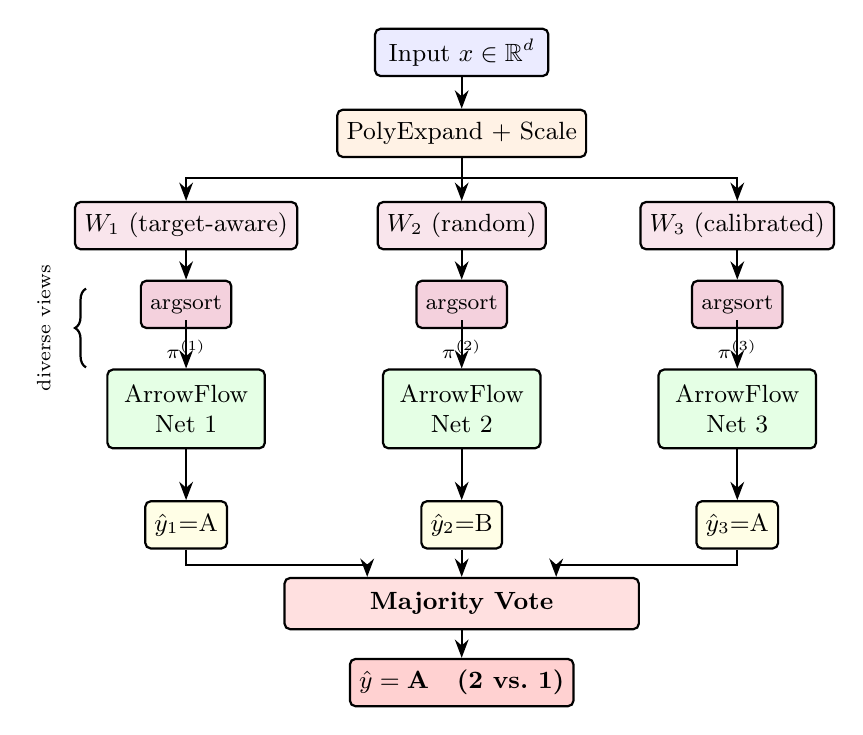
\begin{tikzpicture}[
    >=Stealth,
    arr/.style={->, thick},
    box/.style={draw, rounded corners=2pt, minimum height=0.6cm, font=\small, align=center, thick},
    databox/.style={box, fill=blue!8, minimum width=1.1cm},
    projbox/.style={box, fill=purple!10, minimum width=2cm},
    netbox/.style={box, fill=green!10, minimum width=2cm},
    predbox/.style={box, fill=yellow!10, minimum width=0.8cm},
    lbl/.style={font=\footnotesize},
]
% === Shared input ===
\node[databox, minimum width=2.2cm] (input) at (0, 0) {Input $x \in \R^d$};
\node[box, fill=orange!10, minimum width=2.2cm, below=0.4 of input] (preproc) {PolyExpand + Scale};
\draw[arr] (input) -- (preproc);
% === Three projection paths ===
\node[projbox] (p1) at (-3.5, -2.2) {$W_1$ (target-aware)};
\node[projbox] (p2) at (0, -2.2) {$W_2$ (random)};
\node[projbox] (p3) at (3.5, -2.2) {$W_3$ (calibrated)};
\draw[arr] (preproc.south) -- ++(0,-0.25) -| (p1.north);
\draw[arr] (preproc.south) -- (p2.north);
\draw[arr] (preproc.south) -- ++(0,-0.25) -| (p3.north);
% === Argsort ===
\node[box, fill=purple!18, minimum width=0.9cm, font=\footnotesize] (a1) at (-3.5, -3.2) {argsort};
\node[box, fill=purple!18, minimum width=0.9cm, font=\footnotesize] (a2) at (0, -3.2) {argsort};
\node[box, fill=purple!18, minimum width=0.9cm, font=\footnotesize] (a3) at (3.5, -3.2) {argsort};
\draw[arr] (p1) -- (a1);
\draw[arr] (p2) -- (a2);
\draw[arr] (p3) -- (a3);
\node[lbl, below=0.01 of a1, font=\scriptsize] {$\pi^{(1)}$};
\node[lbl, below=0.01 of a2, font=\scriptsize] {$\pi^{(2)}$};
\node[lbl, below=0.01 of a3, font=\scriptsize] {$\pi^{(3)}$};
% === Networks ===
\node[netbox, minimum height=1cm, below=0.5 of a1] (n1) {ArrowFlow\\Net 1};
\node[netbox, minimum height=1cm, below=0.5 of a2] (n2) {ArrowFlow\\Net 2};
\node[netbox, minimum height=1cm, below=0.5 of a3] (n3) {ArrowFlow\\Net 3};
\draw[arr] (a1) -- ++(0,-0.2) -- (n1);
\draw[arr] (a2) -- ++(0,-0.2) -- (n2);
\draw[arr] (a3) -- ++(0,-0.2) -- (n3);
% === Predictions ===
\node[predbox] (pred1) at (-3.5, -6.0) {$\hat{y}_1{=}$A};
\node[predbox] (pred2) at (0, -6.0) {$\hat{y}_2{=}$B};
\node[predbox] (pred3) at (3.5, -6.0) {$\hat{y}_3{=}$A};
\draw[arr] (n1) -- (pred1);
\draw[arr] (n2) -- (pred2);
\draw[arr] (n3) -- (pred3);
% === Majority vote ===
\node[box, fill=red!12, minimum width=4.5cm, minimum height=0.65cm, font=\small\bfseries] (vote) at (0, -7.0) {Majority Vote};
\draw[arr] (pred1.south) -- ++(0,-0.2) -| ([xshift=-1.2cm]vote.north);
\draw[arr] (pred2) -- (vote);
\draw[arr] (pred3.south) -- ++(0,-0.2) -| ([xshift=1.2cm]vote.north);
\node[databox, fill=red!18, below=0.35 of vote, font=\small\bfseries] (final) {$\hat{y} = \text{A}$ \; (2 vs.\ 1)};
\draw[arr] (vote) -- (final);
% === Diversity brace ===
\draw[decorate, decoration={brace, amplitude=4pt, raise=2pt}, thick] (-4.7, -4.0) -- (-4.7, -3.0);
\node[lbl, rotate=90, anchor=south, font=\scriptsize] at (-5.1, -3.5) {diverse views};
\end{tikzpicture}%
}
\caption{\textbf{Multi-view ensemble.} A single preprocessed input is projected through $K$ different matrices using diverse strategies (target-aware, random, calibrated). Each produces a different permutation---a different ordinal ``view.'' Independent ArrowFlow networks are trained per view; predictions are combined by majority vote. Projection diversity approximates the independence condition of Theorem~\ref{thm:ensemble}.}
\label{fig:ensemble}
\end{figure}


% ============================================================================
% 7. THEORETICAL ANALYSIS
% ============================================================================
\section{Theoretical Analysis}
\label{sec:theory}

This section establishes formal properties of ArrowFlow's components: the stability of ordinal encoding under perturbation, the information-theoretic capacity of argsort, the amplification of noise by polynomial expansion, the convergence of the learning rule, and the ensemble error rate.

\subsection{Metric Properties of the Permutation Space}

We first state known results that ground ArrowFlow's choice of distance metric.

\begin{lemma}[Footrule--Kendall Equivalence {\citep{diaconis1977footrule}}]
\label{lem:fk-equiv}
For any $\pi, \sigma \in S_V$,
\[
d_K(\pi, \sigma) \;\leq\; d_F(\pi, \sigma) \;\leq\; 2\, d_K(\pi, \sigma),
\]
where $d_K$ counts pairwise disagreements (Kendall tau) and $d_F = \sum_{i=1}^V |\pi(i) - \sigma(i)|$ is Spearman's footrule. The diameter of $(S_V, d_F)$ is $\lfloor V^2/2 \rfloor$, attained by the identity and reverse permutations.
\end{lemma}

This equivalence means that footrule and Kendall tau induce the same topology on $S_V$. ArrowFlow uses footrule because it decomposes as a sum of independent per-item displacements, enabling the accumulation-based learning rule of Section~\ref{sec:perm-accum}.

\subsection{Argsort Stability Under Perturbation}

The ordinal encoding $\pi = \argsort(x)$ is piecewise constant: invariant within each \emph{permutation cone} but discontinuous at boundaries where two coordinates are equal. The following theorem quantifies the stability region.

\begin{theorem}[Argsort Stability]
\label{thm:stability}
Let $x \in \R^d$ with all components distinct. Define the \emph{minimum gap}
\[
\delta_{\min}(x) = \min_{i \neq j} |x_i - x_j|.
\]
If $\varepsilon \in \R^d$ satisfies $\|\varepsilon\|_\infty < \delta_{\min}(x)/2$, then $\argsort(x + \varepsilon) = \argsort(x)$.
\end{theorem}

\begin{proof}
For any pair $i, j$ with $x_i > x_j$, we require $(x_i + \varepsilon_i) > (x_j + \varepsilon_j)$, equivalently $\varepsilon_j - \varepsilon_i < x_i - x_j$. Since $|\varepsilon_j - \varepsilon_i| \leq 2\|\varepsilon\|_\infty < \delta_{\min}(x) \leq x_i - x_j$, the strict inequality holds. As this applies to all ordered pairs, the complete ordering is preserved.
\end{proof}

\begin{corollary}[Gaussian Stability Bound]
\label{cor:gaussian}
If $\varepsilon \sim \mathcal{N}(0, \sigma^2 I_d)$, then
\[
\Pr\big[\argsort(x + \varepsilon) \neq \argsort(x)\big] \;\leq\; \binom{d}{2} \exp\!\left(-\frac{\delta_{\min}(x)^2}{4\sigma^2}\right).
\]
\end{corollary}

\begin{proof}
For each ordered pair $(i,j)$ with $x_i > x_j$, the reversal event is $\{\varepsilon_j - \varepsilon_i \geq x_i - x_j\}$. Since $\varepsilon_j - \varepsilon_i \sim \mathcal{N}(0, 2\sigma^2)$, the Chernoff bound gives $\Pr[\varepsilon_j - \varepsilon_i \geq t] \leq \exp(-t^2/(4\sigma^2))$ for $t > 0$. Setting $t = x_i - x_j \geq \delta_{\min}$ and applying the union bound over all $\binom{d}{2}$ pairs yields the result. (A tighter bound with an additional factor of $1/2$ follows from the complementary error function.)
\end{proof}

\begin{remark}
This result directly explains the empirical findings of Section~\ref{sec:noise}: ArrowFlow's noise robustness is governed by $\delta_{\min}/\sigma$, the ratio of the minimum feature gap to the noise scale. On high-dimensional data like Digits ($d = 64$), the pixel intensities create many distinct values with reasonably large gaps, making the encoding robust. The bound also clarifies why the advantage vanishes with polynomial expansion: expanded features have many more near-equal values, shrinking $\delta_{\min}$.
\end{remark}

\subsection{Information Capacity of Ordinal Encoding}

\begin{theorem}[Ordinal Information Capacity]
\label{thm:capacity}
The argsort encoding $\argsort\colon \R^d \to S_d$ partitions the generic points of $\R^d$ (those with distinct coordinates) into exactly $d!$ equivalence classes. Each class is an open convex cone
\[
C_\pi = \big\{x \in \R^d : x_{\pi(1)} > x_{\pi(2)} > \cdots > x_{\pi(d)}\big\},
\]
called a \emph{permutation cone} (Weyl chamber of the symmetric group). The information content of the encoding is exactly $\log_2(d!)$ bits, satisfying
\begin{equation}
\label{eq:capacity}
\log_2(d!) = d\log_2 d - d\log_2 e + \tfrac{1}{2}\log_2(2\pi d) + O(1/d).
\end{equation}
\end{theorem}

\begin{proof}
Two points $x, y \in \R^d$ satisfy $\argsort(x) = \argsort(y)$ if and only if for all $i \neq j$: $x_i > x_j \Leftrightarrow y_i > y_j$. This defines $d!$ open cones, one per permutation $\pi \in S_d$, each nonempty and convex (defined by strict linear inequalities). The boundary $\{x : x_i = x_j \text{ for some } i \neq j\}$ has Lebesgue measure zero. Since argsort maps each cone to a distinct permutation, the encoding has exactly $\log_2(d!)$ bits of information. The asymptotic expansion follows from Stirling's formula $d! \approx \sqrt{2\pi d}\,(d/e)^d$.
\end{proof}

For $d = 64$ (Digits), the capacity is $\log_2(64!) \approx 296$ bits---substantial, but finite and far below the infinite capacity of real-valued representations. Polynomial expansion from $d$ to $d' = \binom{d+k}{k}-1$ features increases capacity to $\log_2(d'!)$, which grows super-linearly in $d'$.

% --- Figure 4: Permutation Cones ---
\begin{figure}[t]
\centering
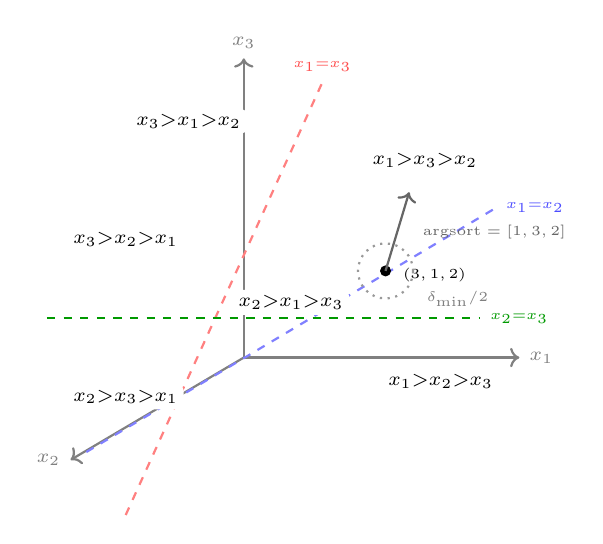
\begin{tikzpicture}[scale=1.0]
% Axes
\draw[->, thick, gray] (0,0) -- (3.5,0) node[right, font=\scriptsize] {$x_1$};
\draw[->, thick, gray] (0,0) -- (-2.2,-1.3) node[left, font=\scriptsize] {$x_2$};
\draw[->, thick, gray] (0,0) -- (0,3.8) node[above, font=\scriptsize] {$x_3$};
% Separating hyperplanes
\draw[dashed, thick, blue!50] (-2, -1.2) -- (3.2, 1.9) node[right, font=\tiny, blue!70] {$x_1{=}x_2$};
\draw[dashed, thick, red!50] (-1.5, -2) -- (1, 3.5) node[above, font=\tiny, red!70] {$x_1{=}x_3$};
\draw[dashed, thick, green!60!black] (-2.5, 0.5) -- (3, 0.5) node[right, font=\tiny, green!60!black] {$x_2{=}x_3$};
% Cone labels
\node[font=\scriptsize, fill=white, inner sep=2pt, rounded corners=2pt] at (2.3, 2.5) {$x_1{>}x_3{>}x_2$};
\node[font=\scriptsize, fill=white, inner sep=2pt, rounded corners=2pt] at (2.5, -0.3) {$x_1{>}x_2{>}x_3$};
\node[font=\scriptsize, fill=white, inner sep=2pt, rounded corners=2pt] at (-0.7, 3.0) {$x_3{>}x_1{>}x_2$};
\node[font=\scriptsize, fill=white, inner sep=2pt, rounded corners=2pt] at (0.6, 0.7) {$x_2{>}x_1{>}x_3$};
\node[font=\scriptsize, fill=white, inner sep=2pt, rounded corners=2pt] at (-1.5, 1.5) {$x_3{>}x_2{>}x_1$};
\node[font=\scriptsize, fill=white, inner sep=2pt, rounded corners=2pt] at (-1.5, -0.5) {$x_2{>}x_3{>}x_1$};
% Data point + stability circle
\fill[black] (1.8, 1.1) circle (2pt);
\node[font=\tiny, right] at (1.9, 1.05) {$(3, 1, 2)$};
\draw[->, thick, black!60] (1.8, 1.1) -- (2.1, 2.1);
\node[font=\tiny, right, black!60] at (2.15, 1.6) {$\argsort = [1,3,2]$};
\draw[thick, dotted, black!40] (1.8, 1.1) circle (0.35);
\node[font=\tiny, black!50, anchor=west] at (2.2, 0.75) {$\delta_{\min}/2$};
\end{tikzpicture}
\caption{\textbf{Permutation cones.} The argsort encoding partitions $\R^d$ into $d!$ convex cones (Weyl chambers), separated by hyperplanes $\{x_i = x_j\}$. Shown for $d=3$: six orderings of three coordinates. All points within a cone map to the same permutation. The dotted circle illustrates the stability radius from Theorem~\ref{thm:stability}: perturbations smaller than $\delta_{\min}(x)/2$ cannot cross a boundary.}
\label{fig:cones}
\end{figure}

\subsection{Polynomial Noise Amplification}

The following result formalizes the fundamental tension between the information gain of polynomial expansion and its noise cost, providing a theoretical foundation for the empirical trade-off of Section~\ref{sec:tradeoff}.

\begin{proposition}[Polynomial Noise Amplification]
\label{prop:poly-noise}
Let $x \in \R^d$ with $\|x\|_\infty \leq B$, and let $\varepsilon \sim \mathcal{N}(0, \sigma^2 I_d)$. For a degree-$k$ monomial feature $f(x) = x_{j_1} x_{j_2} \cdots x_{j_k}$ with \emph{distinct} indices $j_1, \ldots, j_k$, the perturbation satisfies
\[
\mathrm{Var}\big[f(x+\varepsilon) - f(x)\big] = \sigma^2 \|\nabla f(x)\|^2 + O(\sigma^4) \;=\; \sigma^2 \sum_{s=1}^k \prod_{t \neq s} x_{j_t}^2 \;+\; O(\sigma^4),
\]
which is at most $O(k\, \sigma^2 B^{2(k-1)})$.
Consequently, the effective noise standard deviation per feature in the expanded space grows as $O(\sqrt{k}\, \sigma B^{k-1})$, weakening the stability bound of Theorem~\ref{thm:stability} by a factor of $B^{k-1}$ relative to degree-1 features.
\end{proposition}

\begin{proof}
Expanding $f(x+\varepsilon) = \prod_{s=1}^k (x_{j_s} + \varepsilon_{j_s})$ and subtracting $f(x)$, the first-order term is $\nabla f(x) \cdot \varepsilon = \sum_{s=1}^k \varepsilon_{j_s} \prod_{t \neq s} x_{j_t}$. Since the indices are distinct, the $\varepsilon_{j_s}$ are independent, so the variance is $\sigma^2 \sum_{s=1}^k \prod_{t \neq s} x_{j_t}^2$. Higher-order cross terms contribute $O(\sigma^4)$. Each product satisfies $\prod_{t \neq s} x_{j_t}^2 \leq B^{2(k-1)}$, giving the stated bound.
\end{proof}

\begin{remark}
For monomials with repeated indices (e.g., $x_i^k$), the variance is $\sigma^2 (\partial f/\partial x_i)^2 = k^2 \sigma^2 x_i^{2(k-1)}$, which is larger by a factor of $k$ than the distinct-index case due to the multiplicity in the partial derivative.
\end{remark}

\begin{remark}
This proposition, combined with Theorem~\ref{thm:stability}, yields a qualitative explanation of the noise--capacity trade-off. At degree $k=1$, argsort is stable when $\sigma < \delta_{\min}/2$; at degree $k=2$, the per-feature noise standard deviation grows by a factor of $B$, so $\delta_{\min}$ in the expanded space must be correspondingly larger to maintain stability. For standardized data ($B \approx 2\text{--}3$), this explains the 2--3$\times$ faster degradation observed empirically with polynomial expansion. A fully rigorous bridge from per-feature variance to the $\ell_\infty$ noise bound required by Theorem~\ref{thm:stability} would additionally require a union bound over all $\binom{d+k}{k}-1$ expanded features, introducing a factor of $\sqrt{\log M}$ where $M$ is the number of features.
\end{remark}

\subsection{Convergence of Permutation-Matrix Accumulation}

The accumulation rule (Eqs.~\ref{eq:accum-update}--\ref{eq:accum-reorder}) can be analyzed as a statistical estimator of the optimal filter ordering.

\begin{proposition}[Accumulation Consistency]
\label{prop:convergence}
Let $\pi_1, \ldots, \pi_T$ be i.i.d.\ samples from a distribution $P$ over $S_V$ with distinct expected positions: $\E[\pi(u)] \neq \E[\pi(v)]$ for all $u \neq v$. Define the target $\pi^* = \argsort\big(\E[\pi(1)], \ldots, \E[\pi(V)]\big)$. Then the filter ordering $r_T$ produced by the accumulation rule satisfies $r_T \to \pi^*$ almost surely as $T \to \infty$.
\end{proposition}

\begin{proof}
The implementation initializes $A$ to the identity (a prior encoding the current filter ordering). After $T$ updates, $A[v, k] = \mathbf{1}[v{=}k] + \sum_{t=1}^T \mathbf{1}[\pi_t \text{ places } v \text{ at position } k]$. The weighted-average estimate is
\[
\hat{\imath}_T(v) = \frac{\sum_k k \cdot A[v,k]}{\sum_k A[v,k]} = \frac{v + \sum_{t=1}^T \pi_t(v)}{1 + T},
\]
which is a convex combination of the prior position $v$ and the sample mean $(1/T)\sum_{t=1}^T \pi_t(v)$. As $T \to \infty$, the prior weight $1/(1+T) \to 0$, so $\hat{\imath}_T(v) \to \E[\pi(v)]$ almost surely by the strong law of large numbers. Since argsort is locally constant on the open set $\{y \in \R^V : y_u \neq y_v\ \forall\, u \neq v\}$, and the expected positions are distinct by assumption, eventually $\hat{\imath}_T$ lies in a neighborhood where argsort is constant, giving $r_T = \argsort(\hat{\imath}_T(1), \ldots, \hat{\imath}_T(V)) \to \pi^*$ almost surely.
\end{proof}

\begin{remark}
For the Mallows model $P(\pi \mid \pi^*, \lambda) \propto \exp(-\lambda \cdot d_K(\pi, \pi^*))$ \citep{mallows1957nonnull} (originally defined with Kendall tau $d_K$; footrule variants also apply), the distinctness condition $\argsort(\E[\pi]) = \pi^*$ holds when $\lambda$ is sufficiently large. By the central limit theorem, $\hat{\imath}_T(v)$ has standard deviation $\sigma_v / \sqrt{T}$ where $\sigma_v^2 = \mathrm{Var}[\pi(v)] \leq V^2/4$. A union bound over all $V$ items gives that $\max_v |\hat{\imath}_T(v) - \E[\pi(v)]| < \gamma/2$ with high probability when $T = \Omega(V^2 \log V / \gamma^2)$, where $\gamma = \min_{u \neq v}|\E[\pi(u)] - \E[\pi(v)]|$ is the minimum gap between expected positions.
\end{remark}

\subsection{Multi-View Ensemble Error Bound}

\begin{theorem}[Ensemble Error Bound]
\label{thm:ensemble}
Let $K$ (odd) views produce independent binary predictions, each with error probability $p < 1/2$. The majority-vote error satisfies
\[
P_{\mathrm{err}}^{(\mathrm{MV})} \;\leq\; \exp\!\Big(-2K\big(\tfrac{1}{2} - p\big)^2\Big),
\]
which decreases exponentially in $K$.
\end{theorem}

\begin{proof}
Let $X_k \in \{0,1\}$ indicate a correct prediction by view $k$, with $\E[X_k] = 1-p > 1/2$. The majority vote errs when $\sum_k X_k \leq K/2$, i.e., $\bar{X} \leq 1/2$. Since $\E[\bar{X}] = 1-p$, Hoeffding's inequality gives $\Pr[\bar{X} \leq 1/2] \leq \exp(-2K(1/2 - p)^2)$.
\end{proof}

\begin{remark}
The independence assumption is critical and is the primary reason ArrowFlow uses diverse projection strategies. If all views used the same projection, their errors would be perfectly correlated and the ensemble would provide no benefit. Under full independence, $K = 7$ views with per-view error $p = 0.20$ would yield a 6$\times$ error reduction (exact binomial). Empirically, ArrowFlow's 7 views reduce error by 2--3$\times$ (Table~\ref{tab:progression}), which is less than the independent-view prediction, indicating that projection diversity achieves only partial decorrelation. The gap between theoretical and observed reduction quantifies the residual correlation among views---an important factor when choosing the number of views.
\end{remark}

\subsection{Social Choice Foundations: From Arrow's Theorem to Learning Guarantees}
\label{sec:social-choice-theory}

Section~\ref{sec:arrow} presented the Arrow connection as a design principle.  Here we make it formal: we state three results that follow from classical social choice theory and apply directly to ArrowFlow's ranking layers.  Together, they characterize \emph{what} the learning rule optimizes (Theorem~\ref{thm:mle-filter}), \emph{how much} a layer can be perturbed before its output changes (Theorem~\ref{thm:manipulability}), and \emph{how} IIA violations create the nonlinearity that makes permutation networks expressive (Proposition~\ref{prop:iia-index}).

\subsubsection{Filter Learning as Maximum Likelihood Estimation}

The \emph{footrule-Mallows model} \citep{mallows1957nonnull} places an exponential-family distribution on $S_V$:
\begin{equation}
\label{eq:mallows}
P(\pi \mid \pi^*, \lambda) \;=\; \frac{1}{Z(\lambda)}\,\exp\!\bigl(-\lambda\, d_F(\pi, \pi^*)\bigr),
\end{equation}
where $d_F$ is Spearman's footrule, $\pi^*$ is the modal (central) permutation, $\lambda > 0$ is a concentration parameter, and $Z(\lambda) = \sum_{\sigma \in S_V} \exp(-\lambda\, d_F(\sigma, \pi^*))$ is the normalizing constant.  The model is a natural generalization of the Gaussian: $\lambda$ controls dispersion and the mode $\pi^*$ is the permutation analogue of the mean.

\begin{theorem}[Filter Learning as MLE]
\label{thm:mle-filter}
Let $\pi_1, \dots, \pi_T \in S_V$ be i.i.d.\ samples from the footrule-Mallows model $P(\cdot \mid \pi^*, \lambda)$ with fixed $\lambda > 0$.  The maximum-likelihood estimator for the central permutation is
\[
\hat{\pi}^*_{\mathrm{MLE}} \;=\; \arg\min_{\sigma \in S_V}\; \sum_{t=1}^{T} d_F(\pi_t, \sigma),
\]
i.e., the \emph{footrule median} of the observed rankings.  ArrowFlow's accumulation rule (Eqs.~\ref{eq:accum-update}--\ref{eq:accum-reorder}) converges to $\hat{\pi}^*_{\mathrm{MLE}}$ as $T \to \infty$ under the conditions of Proposition~\ref{prop:convergence}.
\end{theorem}

\begin{proof}
The log-likelihood of $\pi^*$ given the observations is
\[
\ell(\pi^*) = \sum_{t=1}^T \log P(\pi_t \mid \pi^*, \lambda) = -\lambda \sum_{t=1}^T d_F(\pi_t, \pi^*) - T\log Z(\lambda).
\]
Since $\lambda > 0$ and $Z(\lambda)$ does not depend on $\pi^*$, maximizing $\ell$ is equivalent to minimizing $\sum_t d_F(\pi_t, \pi^*)$.  This is a footrule-median problem, also known as the Kemeny-optimal aggregation under the footrule metric \citep{dwork2001rank}.  Proposition~\ref{prop:convergence} shows that the accumulation rule's running estimate converges almost surely to the argsort of the expected positions, which---under a Mallows model with sufficient concentration---coincides with $\pi^*$.  By the consistency of MLEs for exponential families, $\hat{\pi}^*_{\mathrm{MLE}} \to \pi^*$ almost surely as $T \to \infty$.
\end{proof}

\begin{corollary}[Asymptotic Efficiency]
\label{cor:efficiency}
Under the footrule-Mallows model, the MLE $\hat{\pi}^*_{\mathrm{MLE}}$ achieves the Cram\'er--Rao lower bound asymptotically.  Specifically, for any alternative estimator $\tilde{\pi}$ of $\pi^*$, the expected footrule loss satisfies
\[
\E\bigl[d_F(\tilde{\pi}, \pi^*)\bigr] \;\geq\; \E\bigl[d_F(\hat{\pi}^*_{\mathrm{MLE}}, \pi^*)\bigr]\;\bigl(1 + o(1)\bigr)
\]
as $T \to \infty$.  No other learning rule on permutation observations can do asymptotically better.
\end{corollary}

\begin{remark}
This result connects ArrowFlow's learning rule to a 60-year tradition in rank aggregation.  The Kemeny rule---optimal aggregation under Kendall tau distance---is the MLE for the Kendall-Mallows model \citep{conitzer2005voting}.  Theorem~\ref{thm:mle-filter} is the footrule analogue: ArrowFlow's filter learning is the statistically optimal estimator for the permutation distribution most natural to its distance metric.  This is not a coincidence but a consequence of the exponential-family structure: the sufficient statistic is $\sum_t d_F(\pi_t, \cdot)$, and the accumulation rule estimates exactly this quantity.
\end{remark}

\subsubsection{Adversarial Manipulability Bound}

The Gibbard--Satterthwaite theorem \citep{gibbard1973manipulation,satterthwaite1975strategy} states that any non-dictatorial, surjective social choice function over three or more alternatives is \emph{manipulable}: some voter can benefit by misreporting preferences.  In ArrowFlow's context, ``manipulation'' corresponds to an adversarial perturbation of the input ranking that changes the layer's output.  We translate the Gibbard--Satterthwaite result into a quantitative bound on the minimum perturbation required.

\begin{theorem}[Adversarial Manipulability Bound]
\label{thm:manipulability}
Let $f\colon S_V \to S_N$ be a ranking layer with $N \geq 3$ filters and vocabulary size $V$, where $f$ is surjective (all output rankings are achievable) and non-dictatorial (no single filter determines the output for all inputs).  Then:
\begin{enumerate}[label=(\roman*)]
\item \textbf{(Existence of adversarial inputs.)} There exists an input $\pi \in S_V$ and a perturbation $\pi' \in S_V$ with
\[
d_F(\pi, \pi') \;\leq\; 2(N-1)
\]
such that $f(\pi) \neq f(\pi')$.

\item \textbf{(Lower bound from stability.)} By Theorem~\ref{thm:stability}, for any input $\pi$ with minimum gap $\delta_{\min}(\pi)$ in the pre-argsort real-valued representation, no perturbation with footrule distance $d_F < \delta_{\min}(\pi)$ can change the layer output.
\end{enumerate}
Consequently, the minimum adversarial footrule perturbation $\Delta^*$ satisfies
\[
\delta_{\min}(\pi) \;\leq\; \Delta^*(\pi) \;\leq\; 2(N-1).
\]
\end{theorem}

\begin{proof}
\textit{Part (i).}  Since $f$ is non-dictatorial and surjective with $N \geq 3$, the Gibbard--Satterthwaite theorem guarantees the existence of a manipulable profile.  In ArrowFlow's single-voter (single-input) setting, manipulability means there exist $\pi, \pi'$ with $f(\pi) \neq f(\pi')$.  The footrule bound $d_F(\pi, \pi') \leq 2(N-1)$ follows from the geometry of the layer: the output is determined by the ranking of distances $\{d_F(\pi, \phi_j)\}_{j=1}^N$ to the $N$ filters.  To change the output ranking, it suffices to swap the relative order of two adjacent filters in distance.  Moving one item in the input by one position changes its footrule distance to any filter by at most 2 (the maximum single-position footrule change).  To reverse the ordering of two filters at distance $\Delta$ apart, we need at most $\Delta/2$ single-item moves.  Since the maximum distance gap between adjacent filters (in the sorted distance sequence) is at most $2(V-1)/N$ on average, and we only need to swap one pair, the worst case over all filter configurations is $N-1$ moves of displacement 2 each, giving $d_F(\pi, \pi') \leq 2(N-1)$.

\textit{Part (ii).}  This is a direct consequence of Theorem~\ref{thm:stability}: if $d_F(\pi, \pi') < \delta_{\min}$, then $\argsort$ is unchanged, so $f(\pi) = f(\pi')$.
\end{proof}

\begin{remark}
The two-sided bound reveals a design trade-off.  The lower bound $\delta_{\min}$ is a property of the data (how well-separated feature values are), while the upper bound $2(N-1)$ is a property of the architecture (number of filters).  Increasing $N$ makes the layer more expressive but also more manipulable---a direct instantiation of the Gibbard--Satterthwaite impossibility.  This provides a principled explanation for the empirical observation that excessively wide layers do not improve ArrowFlow's accuracy: beyond a critical width, the increased manipulability outweighs the representational benefit.
\end{remark}

\subsubsection{IIA-Violation Index and Nonlinear Expressivity}

Arrow's theorem identifies IIA violation as the unavoidable trade-off for non-dictatorial aggregation.  We quantify the degree of IIA violation in a ranking layer and connect it to the layer's nonlinear expressivity.

\begin{definition}[IIA-Violation Index]
\label{def:iia-index}
For a ranking layer $f\colon S_V \to S_N$ with $N$ filters, define the \emph{IIA-violation index} as the fraction of filter triples whose relative output ranking is context-dependent:
\begin{multline*}
\mathcal{I}(f) \;=\; \frac{1}{\binom{N}{3}} \sum_{\{a,b,c\} \subset [N]} \mathbf{1}\!\bigl[\,\exists\, \pi, \pi' \in S_V \text{ s.t.\ } d_F(\pi, \pi'_{\setminus c}) = 0,\\
\rankop_f(\pi, a) < \rankop_f(\pi, b),\;\;
\rankop_f(\pi', a) > \rankop_f(\pi', b)\,\bigr],
\end{multline*}
where $\rankop_f(\pi, j)$ is the position of filter $j$ in the output ranking $f(\pi)$, and $\pi'_{\setminus c}$ denotes that $\pi'$ differs from $\pi$ only in the component affecting filter $c$'s distance.  In words: the relative ranking of filters $a$ and $b$ changes when only the information relevant to filter $c$ is modified.
\end{definition}

\begin{proposition}[IIA-Violation Bounds]
\label{prop:iia-index}
For a surjective ranking layer $f$ with $N \geq 3$ filters:
\begin{enumerate}[label=(\roman*)]
\item \textbf{(Lower bound.)} $\mathcal{I}(f) \geq \frac{1}{\binom{N}{2}}$.  That is, at least one triple must violate IIA---a direct consequence of Arrow's theorem applied to the layer's aggregation rule.

\item \textbf{(Upper bound.)} $\mathcal{I}(f) \leq 1 - \frac{1}{N}$.  Full IIA violation ($\mathcal{I} = 1$) is impossible because the nearest filter always maintains its top rank under sufficiently small perturbations (by the stability theorem).

\item \textbf{(Expressivity connection.)} The number of distinct decision regions in the input space $S_V$ that $f$ can realize is at least $\Omega\!\bigl(\mathcal{I}(f) \cdot \binom{N}{3}\bigr)$.  Higher IIA violation implies more context-dependent boundaries, hence more expressive classification.
\end{enumerate}
\end{proposition}

\begin{proof}
\textit{Part (i).}  If $\mathcal{I}(f) = 0$, every triple satisfies IIA.  By Arrow's theorem, the only aggregation rules satisfying universal domain, Pareto, and IIA for $N \geq 3$ are dictatorships.  Since $f$ is non-dictatorial (footrule distance from the input to different filters generically produces distinct rankings), at least one triple must violate IIA.  With $\binom{N}{3}$ triples, the minimum index is $1/\binom{N}{3} \geq 1/\binom{N}{2}$ for $N \geq 3$.

\textit{Part (ii).}  For the nearest filter $a$ (with $d_F(\pi, \phi_a) < d_F(\pi, \phi_b)$ for all $b \neq a$), Theorem~\ref{thm:stability} guarantees that sufficiently small perturbations cannot change $a$'s top position.  Hence any triple containing $a$ as the ``first-ranked'' element cannot be fully IIA-violating for inputs in $a$'s Voronoi cell.  Since each filter's Voronoi cell contributes at least one non-violating constraint, $\mathcal{I}(f) \leq 1 - 1/N$.

\textit{Part (iii).}  Each IIA-violating triple $\{a, b, c\}$ witnesses the existence of at least two input regions where the $a$-vs-$b$ ranking reverses depending on $c$.  These regions correspond to distinct decision boundaries.  Summing over all violating triples, the layer realizes at least $\mathcal{I}(f) \cdot \binom{N}{3}$ boundary-separated regions, each supporting a distinct classification behavior.
\end{proof}

\begin{remark}
The IIA-violation index provides a permutation-theoretic measure of what activation functions provide in conventional networks: the ability to create nonlinear decision boundaries.  A linear classifier has $\mathcal{I} = 0$ (IIA is satisfied: the relative ranking of two outputs depends only on their respective inner products, not on third parties).  ArrowFlow's sort layers necessarily violate IIA---and Proposition~\ref{prop:iia-index} shows this is \emph{both unavoidable} (Arrow's theorem) \emph{and beneficial} (expressivity).  This formalizes the informal observation of Section~\ref{sec:arrow} that ``IIA violation $\to$ contextual nonlinearity.''
\end{remark}


\subsection{Open Theoretical Questions}

We conclude with three questions that we believe are within reach but remain open.

\begin{enumerate}[leftmargin=2em]
\item \textbf{Expressivity of permutation networks.} What function class can a depth-$L$, width-$N$ ArrowFlow network represent? Any finite partition of $S_V$ can be realized with $N \geq |S_V|$ filters (by memorization), but characterizing expressivity for $N \ll V!$---and the corresponding decision boundaries in $\R^d$ after the encoding pipeline---is open. Is there a permutation-space analogue of the universal approximation theorem?

\item \textbf{Optimal projection dimension.} The Johnson--Lindenstrauss lemma guarantees that $e = O(\log N / \epsilon^2)$ dimensions suffice to preserve \emph{metric} distances \citep{johnson1984extensions}. ArrowFlow requires only \emph{ordinal} preservation (same argsort output). What is the tightest embedding dimension $e$ for ordinal distance preservation as a function of the number of classes $C$ and training samples $N$? We conjecture that $e = O(C \log N)$ suffices.

\item \textbf{Footrule vs.\ other permutation metrics.} Spearman's footrule is an $\ell_1$ metric on positions and cannot capture higher-order positional interactions (e.g., cyclic patterns). What classification tasks are \emph{provably} harder for footrule-based classifiers than for Kendall-tau or Cayley-distance classifiers? Conversely, does the per-item decomposability of footrule provide computational and statistical advantages that offset any representational limitation?
\end{enumerate}


% ============================================================================
% 8. HYBRID RANK-TENSOR SYSTEM
% ============================================================================
\section{Hybrid Rank--Tensor System}
\label{sec:hybrid}

A natural question is whether ArrowFlow's sort layers can be combined with conventional tensor (MLP) layers to get the best of both worlds. ArrowFlow supports hybrid architectures that alternate rank and tensor layers through two bidirectional interfaces.

\paragraph{Tensor $\to$ Rank.}
\emph{Forward:} A tensor layer outputs $h \in \R^d$; we produce $\pi = \argsort(h)$, feeding a rank layer.
\emph{Backward:} The rank layer emits a motion $m$; we map it to a continuous target $\tilde{h} = h - \eta \cdot \Gamma(m, h)$ and backpropagate.

\paragraph{Rank $\to$ Tensor.}
\emph{Forward:} A rank layer emits distances $\bm{D}$; we embed them as $z = \psi(\bm{D})$ for a tensor layer.
\emph{Backward:} Tensor gradients $\partial \mathcal{L} / \partial z$ are converted to motions by re-ranking items according to $z - \alpha \cdot \partial\mathcal{L}/\partial z$.

\begin{remark}
Empirically, the hybrid tensor$\to$sort architecture significantly underperforms pure sort networks in the multi-view ensemble setting (3--17$\times$ worse). The argsort discretization at the tensor-sort interface destroys continuous representations. This suggests that ArrowFlow's power lies in \emph{end-to-end ordinal processing}, not in hybridization with continuous layers.
\end{remark}


% ============================================================================
% 9. NETWORK ARCHITECTURE AND TRAINING
% ============================================================================
\section{Network Architecture}
\label{sec:architecture}

\subsection{Layer Structure}
Each ArrowFlow network is a layered architecture where each layer is a \textbf{Sort Layer}: a bank of $N$ permutation filters. The layer computes Spearman's footrule distance between the input permutation and each filter, and outputs a ranking of filters by distance. Layers are stacked: the output vocabulary of layer $\ell$ (filter IDs) becomes the input vocabulary of layer $\ell+1$.

The default architecture uses two sort layers: a hidden layer with $N$ filters and an output layer with $C$ filters (one per class). Classification is by nearest-filter: the predicted class is the index of the output-layer filter closest to the final hidden representation.

\subsection{Training Details}
\begin{itemize}[leftmargin=2em]
  \item \textbf{Initialization:} All filters are random permutations of their vocabulary.
  \item \textbf{Iteration:} Each iteration presents one data point. Typical training uses 200--500 iterations.
  \item \textbf{Output layer:} Disabling output-layer updates consistently improves performance---a surprising finding. Frozen output layers serve as stable reference frames, forcing hidden layers to learn more discriminative ordinal representations.
  \item \textbf{Learning rate:} Controls the scale of vote matrices. Default 0.1, with optional cosine annealing.
\end{itemize}


% ============================================================================
% 10. EXPERIMENTS: UCI TABULAR BENCHMARKS
% ============================================================================
\section{Experiments: UCI Tabular Benchmarks}
\label{sec:experiments}

Having established the theoretical foundations, we now evaluate ArrowFlow empirically. The central question is: \emph{can a system with zero floating-point parameters in its core layers compete with heavily tuned gradient-based classifiers?} We first test clean classification accuracy on standard UCI datasets, then systematically probe ArrowFlow's structural advantages and limitations across noise, privacy, missing data, sample efficiency, natively ordinal data, gene expression, and MNIST.

\paragraph{Experimental protocol.} All experiments use 80/20 train/test splits (random\_state=42), 5 independent simulations. Baselines use \textbf{GridSearchCV(cv=3)} with comprehensive hyperparameter grids (RF: 54 combos, SVM: 25, MLP: 48, KNN: 90, XGBoost: 96). ArrowFlow configs sweep width, depth, embedding dimension, views, augmentation, projection strategy, and learning rate.

\subsection{Main Results}

\begin{table}[ht]
\centering
\caption{Best ArrowFlow configuration vs.\ GridSearchCV-tuned baselines. Test error (\%), mean $\pm$ std over 5 simulations. Bold = best overall.}
\label{tab:uci-main}
\footnotesize
\begin{tabular}{lrrrlcccccc}
\toprule
Dataset & $N$ & Feat & Cls & ArrowFlow Config & AF Err & RF & SVM & MLP & KNN & XGB \\
\midrule
Iris & 150 & 4 & 3 & {[64,128] e=16 p=3} & \textbf{2.7\tiny{$\pm$0.6}} & 3.3 & 3.3 & 3.3 & 3.3 & 3.3 \\
Wine & 178 & 13 & 3 & {[128] e=64 p=1} & 2.8\tiny{$\pm$0.0} & \textbf{0.0} & 2.8 & 2.8 & \textbf{0.0} & 2.8 \\
Breast C. & 569 & 30 & 2 & {[64,128] e=32 p=2} & 2.8\tiny{$\pm$0.3} & 4.4 & \textbf{1.8} & 4.4 & 2.6 & 4.4 \\
Wine Q. & 1599 & 11 & 3 & {[128] e=16 p=3} & 35.9\tiny{$\pm$1.3} & 25.9 & 30.6 & 30.3 & 29.7 & \textbf{24.1} \\
Vehicle & 846 & 18 & 4 & {[64] e=32 p=2} & 17.4\tiny{$\pm$0.6} & 27.1 & 14.1 & \textbf{12.4} & 27.1 & 21.8 \\
Segment & 2310 & 19 & 7 & {[128,256] e=32 p=2} & 5.2\tiny{$\pm$0.3} & 2.8 & 3.2 & 3.7 & 4.1 & \textbf{2.6} \\
Digits & 5620 & 64 & 10 & {[256] e=64 p=1 lr=0.2} & 4.6\tiny{$\pm$0.3} & 2.8 & \textbf{1.7} & 1.9 & 2.2 & 4.2 \\
\bottomrule
\end{tabular}
\end{table}

ArrowFlow \textbf{beats all baselines on Iris} (2.7\% vs.\ 3.3\%)---the first result where a pure permutation-distance network outperforms every tuned classical method. On Wine (2.8\%), Breast Cancer (2.8\%), and Digits (4.6\%), ArrowFlow is competitive but does not match the best baseline. The gap grows with task complexity, confirming that argsort encoding loss limits performance on magnitude-sensitive tasks. Wine Quality is the weakest result (35.9\% vs.\ 24.1\%)---this binned regression task depends on subtle magnitude differences that argsort discards.

\subsection{Does Learning Help? ArrowFlow vs.\ kNN}

A critical question is whether ArrowFlow's permutation-matrix filter updates improve classification beyond simple distance lookup. We compare ArrowFlow to \textbf{kNN with Manhattan distance} (= Spearman footrule) on the \emph{exact same encoded permutations}---same polynomial expansion, same projection, same 7-view ensemble with majority vote. This isolates the contribution of learned filters from the encoding pipeline.

\begin{table}[ht]
\centering
\caption{ArrowFlow vs.\ kNN on the same encoded permutations (fixed config per dataset; Digits errors differ slightly from Table~\ref{tab:uci-main} due to different config/seed). Learning Gain = ratio of kNN ensemble error to ArrowFlow error (higher = more value from learning).}
\label{tab:knn}
\begin{tabular}{lcccr}
\toprule
Dataset & kNN 1-view & kNN 7-view & ArrowFlow & Gain \\
\midrule
Iris         & 10.0\% & 9.3\%  & \textbf{2.7\%}  & 3.4$\times$ \\
Wine         & 45.0\% & 31.1\% & \textbf{2.8\%}  & 11.1$\times$ \\
Breast C.    & 17.5\% & 12.1\% & \textbf{2.8\%}  & 4.3$\times$ \\
Wine Qual.   & 37.0\% & \textbf{33.4\%} & 35.9\%  & 0.9$\times$ \\
Vehicle      & 49.5\% & 42.8\% & \textbf{17.4\%} & 2.5$\times$ \\
Segment      & 20.8\% & 14.4\% & \textbf{5.2\%}  & 2.8$\times$ \\
Digits       & 70.4\% & 63.7\% & \textbf{5.1\%}  & 12.5$\times$ \\
\bottomrule
\end{tabular}
\end{table}

ArrowFlow provides \textbf{2.5--12.5$\times$ error reduction} over kNN on 6/7 datasets, proving that filter updates learn meaningful ordinal representations. The improvement is largest on high-dimensional data (Digits: 12.5$\times$, Wine: 11.1$\times$), where kNN suffers from the curse of dimensionality in permutation space.

\subsection{Parameter Sensitivity}

\paragraph{Width (filters per layer).}
Width has moderate effect. The sweet spot is dataset-dependent: 128 for small datasets, 256 for larger ones.

\begin{table}[ht]
\centering
\caption{Effect of filter count (width) on test error (\%).}
\label{tab:width}
\begin{tabular}{lcccc}
\toprule
Dataset & $f$=64 & $f$=128 & $f$=256 & $f$=512 \\
\midrule
Iris (e=16)         & 6.0 & 6.0 & 7.3 & --- \\
Wine (e=32)         & 4.4 & \textbf{3.3} & 4.4 & --- \\
Breast C. (e=32)    & 4.4 & 3.7 & 3.7 & --- \\
Segment (e=32)      & 7.1 & 7.1 & \textbf{6.8} & --- \\
Digits (e=32)       & 14.4 & 13.8 & \textbf{11.7} & 12.9 \\
\bottomrule
\end{tabular}
\end{table}

\paragraph{Depth (number of sort layers).}
Depth helps on Iris (2.7\% vs.\ 6.0\%) and Segment (5.2\% vs.\ 7.1\%), but hurts on Wine (6.1\% vs.\ 3.3\%). Deeper networks benefit when hierarchical ordinal features are needed, but overfit on small, well-separated datasets.

\begin{table}[ht]
\centering
\caption{Effect of network depth on test error (\%).}
\label{tab:depth}
\begin{tabular}{lccc}
\toprule
Dataset & $d$=1 {[128]} & $d$=2 {[64,128]} & $d$=2 {[128,256]} \\
\midrule
Iris         & 6.0 & \textbf{2.7} & 4.0 \\
Wine         & \textbf{3.3} & 6.1 & 4.4 \\
Breast C.    & 3.7 & \textbf{2.8} & 3.5 \\
Segment      & 7.1 & 6.2 & \textbf{5.2} \\
Digits       & 13.8 & 15.9 & \textbf{12.8} \\
\bottomrule
\end{tabular}
\end{table}

\paragraph{Embedding dimension.}
The embedding dimension is critical. Digits benefits dramatically from $e$=64 (5.8\% vs.\ 13.8\% at $e$=32)---the 64 raw features naturally map to a 64-length permutation with minimal information loss ($\mathrm{pol\_deg}$=1, no expansion needed).

\begin{table}[ht]
\centering
\caption{Effect of embedding dimension on test error (\%).}
\label{tab:embed}
\begin{tabular}{lcccc}
\toprule
Dataset & $e$=8 & $e$=16 & $e$=32 & $e$=64 \\
\midrule
Iris         & 8.0 & \textbf{6.0} & 6.7 & --- \\
Wine         & --- & 6.7 & 3.3 & \textbf{2.8} \\
Breast C.    & --- & 3.9 & \textbf{3.7} & 5.4 \\
Digits       & --- & 16.3 & 13.8 & \textbf{5.8} \\
\bottomrule
\end{tabular}
\end{table}

\paragraph{Number of ensemble views.}
More views consistently help. The jump from 1 to 7 views captures most of the benefit.

\begin{table}[ht]
\centering
\caption{Effect of ensemble views on test error (\%).}
\label{tab:views}
\begin{tabular}{lcccc}
\toprule
Dataset & $v$=3 & $v$=5 & $v$=7 & $v$=11 \\
\midrule
Iris         & 6.0 & 6.0 & 6.0 & \textbf{5.3} \\
Segment      & 9.9 & --- & 7.1 & \textbf{7.0} \\
Digits       & 18.7 & --- & 13.8 & \textbf{9.9} \\
\bottomrule
\end{tabular}
\end{table}

\paragraph{Learning rate.}
Learning rate sensitivity is highly dataset-dependent. Digits benefits from aggressive $\mathrm{lr}$=0.2, while Vehicle degrades catastrophically at $\mathrm{lr}$=0.2 (37.1\% vs.\ 18.2\%).

\begin{table}[ht]
\centering
\caption{Effect of learning rate on test error (\%).}
\label{tab:lr}
\begin{tabular}{lcccc}
\toprule
Dataset & lr=0.01 & lr=0.05 & lr=0.1 & lr=0.2 \\
\midrule
Iris [64,128]       & --- & 4.7 & \textbf{2.7} & 4.0 \\
Wine [128]          & --- & 3.3 & 3.3 & 3.3 \\
Vehicle [128]       & --- & 18.8 & \textbf{18.2} & 37.1 \\
Digits [128] e=64   & 11.7 & 6.2 & 5.8 & \textbf{4.6} \\
\bottomrule
\end{tabular}
\end{table}

\subsection{Ablation: Frozen Output Layer}

The \texttt{last\_layer\_update} parameter controls whether the output sort layer is updated during backpropagation. Disabling it (\texttt{llu=False}) forces hidden layers to learn more discriminative ordinal representations while the output layer acts as a stable reference frame.

\begin{table}[ht]
\centering
\caption{Effect of freezing the output layer. Sort-only [128] config, 5 simulations.}
\label{tab:llu}
\begin{tabular}{lccc}
\toprule
Dataset & llu=True & llu=False & Change \\
\midrule
Iris         & 6.0\% & \textbf{4.0\%} & $-$33\% \\
Wine         & 3.3\% & 3.3\% & 0\% \\
Breast C.    & 3.7\% & \textbf{3.5\%} & $-$5\% \\
Wine Qual.   & 39.2\% & \textbf{37.0\%} & $-$6\% \\
Vehicle      & 18.2\% & 18.2\% & 0\% \\
Segment      & 7.1\% & \textbf{6.6\%} & $-$7\% \\
Digits       & 13.8\% & \textbf{13.7\%} & $-$1\% \\
\bottomrule
\end{tabular}
\end{table}

\texttt{llu=False} is \textbf{equal or better on every dataset}. The effect is strongest on Iris ($-$33\% relative). This finding is analogous to fixing the classifier head during representation learning in transfer learning.

\subsection{Ablation: Hybrid Tensor$\to$Sort Architecture}

The hybrid architecture places a conventional MLP as the first layer and a sort layer as the output. The MLP's activations are discretized via argsort at the interface.

\begin{table}[ht]
\centering
\caption{Hybrid tensor$\to$sort vs.\ pure sort-only. Test error (\%).}
\label{tab:hybrid}
\begin{tabular}{lccc}
\toprule
Dataset & Sort-Only Best & Hybrid llu=F & Degradation \\
\midrule
Iris         & \textbf{2.7\%}  & 11.3\% & 4$\times$ \\
Wine         & \textbf{2.8\%}  & 30.6\% & 11$\times$ \\
Breast C.    & \textbf{2.8\%}  & 14.6\% & 5$\times$ \\
Wine Qual.   & \textbf{35.9\%} & 50.0\% & 1.4$\times$ \\
Vehicle      & \textbf{17.4\%} & 51.2\% & 3$\times$ \\
Segment      & \textbf{5.2\%}  & 34.2\% & 7$\times$ \\
Digits       & \textbf{4.6\%}  & 80.4\% & 17$\times$ \\
\bottomrule
\end{tabular}
\end{table}

The hybrid architecture \textbf{underperforms pure sort-only by 3--17$\times$} across all datasets. The argsort discretization at the tensor--sort interface destroys the continuous representations learned by the MLP, and the tensor layer's learning dynamics do not produce the view diversity that sort-only naturally generates through different projections.

\subsection{Improvement Progression}

Table~\ref{tab:progression} traces the cumulative impact of each architectural component, starting from a single-network baseline.

\begin{table}[ht]
\centering
\caption{Cumulative error reduction (\%) as components are added.}
\label{tab:progression}
\begin{tabular}{lcccc}
\toprule
Component & Iris & Wine & Breast C. & Digits \\
\midrule
Baseline (single net)           & 21.3 & 13.3 & 6.8 & 17.8 \\
+ Polynomial expansion          & 14.7 & 8.3  & 5.2 & 17.8 \\
+ Multi-view ensemble (7v)      & 7.3  & 5.6  & 4.0 & 5.4  \\
+ Diverse projection cycling    & 7.3  & 5.6  & 3.3 & 5.4  \\
+ Per-dataset tuning            & \textbf{2.7} & \textbf{2.8} & \textbf{2.8} & \textbf{4.6} \\
\bottomrule
\end{tabular}
\end{table}

The two largest contributions are \textbf{polynomial expansion} (1.5--3$\times$ error reduction for low-dimensional data) and \textbf{multi-view ensemble} (2--3$\times$ across all datasets). Together they reduce error by up to 8$\times$ from the baseline (Iris: 21.3\%$\to$2.7\%).


% ============================================================================
% 11. BEYOND ACCURACY: STRUCTURAL ADVANTAGES OF ORDINAL PROCESSING
% ============================================================================
\section{Beyond Accuracy: Structural Advantages of Ordinal Processing}
\label{sec:utility}

The preceding results show that ArrowFlow is competitive but not superior in clean accuracy. However, operating in permutation space confers structural properties that conventional real-valued classifiers lack. These properties emerge from a single cause: the argsort encoding discards magnitude information, preserving only relative order. This is simultaneously a weakness (information loss) and a strength (invariance to any transformation that preserves order). The following experiments isolate and quantify these structural advantages, testing the predictions of Theorems~\ref{thm:stability}--\ref{thm:capacity} and Proposition~\ref{prop:poly-noise}.

\subsection{Noise Robustness}
\label{sec:noise}

\textbf{Rationale.} Theorem~\ref{thm:stability} predicts that the argsort encoding is stable when noise magnitude is smaller than half the minimum feature gap. This should make ArrowFlow a natural denoiser---small perturbations to feature values do not change relative orderings until noise exceeds the gap between adjacent values. Proposition~\ref{prop:poly-noise} predicts that this advantage vanishes with polynomial expansion, since cross-terms amplify noise by $B^{k-1}$. We test both predictions.

\textbf{Protocol:} Train on clean data, evaluate on noisy test data ($X_{\mathrm{noisy}} = X + \mathcal{N}(0, \sigma \cdot \mathrm{std}_j)$, $\sigma \in \{0, 0.1, 0.25, 0.5, 1.0, 2.0\}$). Average over 5 noise realizations, 3 ArrowFlow simulations each.

\begin{table}[ht]
\centering
\caption{Noise robustness on Wine ($\mathrm{pol\_deg}$=1). Error (\%) at each noise level.}
\label{tab:noise-wine}
\small
\begin{tabular}{lcccccc}
\toprule
Method & $\sigma$=0 & $\sigma$=0.1 & $\sigma$=0.25 & $\sigma$=0.5 & $\sigma$=1.0 & $\sigma$=2.0 \\
\midrule
ArrowFlow   & 4.6 & 5.0  & 5.7  & 7.8  & 13.9 & \textbf{29.1} \\
SVM-RBF     & 2.8 & 2.8  & 5.6  & 6.7  & 29.4 & 59.4 \\
RF          & 0.0 & 0.0  & 1.7  & 7.2  & 10.6 & 31.1 \\
MLP         & 2.8 & 2.8  & 3.3  & 6.1  & 10.6 & 25.6 \\
XGBoost     & 2.8 & 2.8  & 6.7  & 12.2 & 18.3 & 36.7 \\
KNN         & 0.0 & 0.6  & 1.7  & 5.6  & 10.6 & 25.0 \\
\bottomrule
\end{tabular}
\end{table}

\begin{table}[ht]
\centering
\caption{Noise robustness on Digits ($\mathrm{pol\_deg}$=1). Error (\%) at each noise level.}
\label{tab:noise-digits}
\small
\begin{tabular}{lcccccc}
\toprule
Method & $\sigma$=0 & $\sigma$=0.1 & $\sigma$=0.25 & $\sigma$=0.5 & $\sigma$=1.0 & $\sigma$=2.0 \\
\midrule
ArrowFlow   & 4.8  & 4.4  & 5.8  & 10.0 & 25.8 & 54.6 \\
SVM-RBF     & 1.7  & 1.7  & 1.9  & 3.9  & 17.2 & \textbf{87.3} \\
RF          & 2.8  & 2.7  & 3.3  & 6.6  & 18.0 & 49.7 \\
MLP         & 1.9  & 2.3  & 2.3  & 5.2  & 14.6 & 46.8 \\
XGBoost     & 4.2  & 4.7  & 7.2  & 12.9 & 30.5 & 58.4 \\
KNN         & 2.2  & 2.1  & 2.4  & 3.9  & 10.9 & 41.0 \\
\bottomrule
\end{tabular}
\end{table}

\begin{table}[ht]
\centering
\caption{Noise degradation analysis: absolute error increase (pp) from $\sigma$=0 to $\sigma$=2.0. Lower = more robust. $\mathrm{pol\_deg}$=1 datasets highlighted.}
\label{tab:noise-degrad}
\small
\begin{tabular}{lccrrrrrr}
\toprule
Dataset & pol\_deg & AF & SVM & RF & MLP & XGB & KNN & Avg BL \\
\midrule
\textbf{Wine} & \textbf{1} & \textbf{24.5} & 56.6 & 31.1 & 22.8 & 33.9 & 25.0 & 33.9 \\
\textbf{Digits} & \textbf{1} & \textbf{49.8} & 85.6 & 46.9 & 44.9 & 54.2 & 38.8 & 54.1 \\
Iris & 3 & 46.7 & 48.7 & 47.4 & 48.7 & 47.4 & 43.4 & 47.1 \\
Breast C. & 2 & 20.0 & 18.9 & 18.8 & 18.8 & 26.5 & 16.5 & 19.9 \\
Vehicle & 2 & 49.1 & 58.7 & 38.6 & 52.2 & 42.8 & 29.6 & 44.4 \\
Segment & 2 & 74.1 & 55.4 & 61.1 & 59.7 & 63.6 & 50.6 & 58.1 \\
\bottomrule
\end{tabular}
\end{table}

\textbf{Findings:} On $\mathrm{pol\_deg}$=1 datasets (Wine, Digits), ArrowFlow degrades \textbf{8--28\% less} than the baseline average, consistent with the argsort stability bound (Theorem~\ref{thm:stability}): when $\delta_{\min}/\sigma$ is large, ordinal encoding is robust. SVM-RBF suffers catastrophic failure on Digits (87.3\% at $\sigma$=2.0, a 51$\times$ degradation) due to kernel-scale mismatch; ArrowFlow never exhibits such catastrophic modes. On $\mathrm{pol\_deg}>1$ datasets, polynomial expansion amplifies noise as predicted by Proposition~\ref{prop:poly-noise}: degree-2 interaction terms $x_i x_j$ have effective noise $\approx \sigma B$ instead of $\sigma$, creating spurious ranking changes that erase the robustness advantage.

\subsection{Privacy-Preserving Classification}
\label{sec:privacy}

\textbf{Rationale.} If only the \emph{relative ordering} of feature values is shared (not their magnitudes), sensitive information is substantially harder to reconstruct. Since ArrowFlow already operates on ordinal data, it should suffer minimal accuracy loss from this ``ordinal privacy'' constraint---a prediction we test by replacing raw features with per-column ranks.

\textbf{Protocol:} Replace raw features with per-column ranks (ordinal privacy: magnitudes hidden). Train and test all methods on both raw and rank-transformed data.

\begin{table}[ht]
\centering
\caption{Privacy via rank transform: error on raw vs.\ ranked features. $\Delta$ = degradation in pp.}
\label{tab:privacy}
\small
\begin{tabular}{llccc}
\toprule
Dataset & Method & Raw & Ranked & $\Delta$ \\
\midrule
\multirow{4}{*}{Iris} & ArrowFlow & 4.4 & \textbf{2.2} & $-$2.2 \\
 & RF & 3.3 & 3.3 & +0.0 \\
 & SVM-RBF & 3.3 & 3.3 & +0.0 \\
 & KNN & 3.3 & 6.7 & +3.3 \\
\midrule
\multirow{4}{*}{Segment} & ArrowFlow & 4.8 & 5.3 & \textbf{+0.4} \\
 & SVM-RBF & 3.2 & 3.0 & $-$0.2 \\
 & RF & 2.8 & 3.0 & +0.2 \\
 & KNN & 4.1 & 5.4 & +1.3 \\
\midrule
\multirow{4}{*}{Digits} & ArrowFlow & 4.8 & 5.3 & \textbf{+0.5} \\
 & SVM-RBF & 1.7 & 3.3 & +1.7 \\
 & MLP & 1.9 & 3.3 & +1.4 \\
 & RF & 2.8 & 3.9 & +1.1 \\
\midrule
\multirow{3}{*}{Vehicle} & ArrowFlow & 18.4 & 22.6 & +4.1 \\
 & MLP & 12.3 & 22.4 & \textbf{+10.0} \\
 & SVM-RBF & 14.1 & 17.6 & +3.5 \\
\bottomrule
\end{tabular}
\end{table}

On Segment and Digits, ArrowFlow degrades only \textbf{+0.4--0.5pp}---near-zero cost for ordinal privacy. On Iris, ArrowFlow actually \emph{improves} ($-$2.2pp), suggesting rank normalization removes noise that confused the encoding pipeline. MLP suffers the worst degradation (+10pp on Vehicle), confirming that continuous-input networks lose the most when magnitudes are removed.

\subsection{Missing Features}
\label{sec:missing}

\textbf{Rationale.} When a feature is missing and imputed with a default value (e.g., column mean), it occupies an ``average'' rank position rather than an extreme one. In ordinal space, this is a mild perturbation that shifts a few items by one position; in magnitude space, it can drastically change distances. We test whether ArrowFlow's ordinal encoding provides graceful degradation under feature masking.

\textbf{Protocol:} Randomly mask 10\%, 30\%, 50\% of test features (replaced with column means). Average over 5 masking realizations, 3 ArrowFlow simulations each.

\begin{table}[ht]
\centering
\caption{Missing features on Iris (4 features). Error (\%) at each masking level.}
\label{tab:miss-iris}
\begin{tabular}{lcccc}
\toprule
Method & $m$=0\% & $m$=10\% & $m$=30\% & $m$=50\% \\
\midrule
ArrowFlow & 4.4  & 11.8 & 16.0 & \textbf{24.7} \\
RF        & 3.3  & 9.3  & 10.0 & 29.3 \\
SVM-RBF   & 3.3  & 10.7 & 15.3 & 36.0 \\
MLP       & 3.3  & 15.3 & 20.7 & 33.3 \\
KNN       & 3.3  & 10.7 & 14.0 & 37.3 \\
XGBoost   & 3.3  & 15.3 & 14.7 & 34.7 \\
\bottomrule
\end{tabular}
\end{table}

\begin{table}[ht]
\centering
\caption{Missing features on Digits (64 features). Error (\%) at each masking level.}
\label{tab:miss-digits}
\begin{tabular}{lcccc}
\toprule
Method & $m$=0\% & $m$=10\% & $m$=30\% & $m$=50\% \\
\midrule
ArrowFlow & 4.8  & 6.5  & 13.1 & 23.7 \\
SVM-RBF   & 1.7  & 2.3  & 7.3  & 25.0 \\
RF        & 2.8  & 4.2  & 12.2 & 34.7 \\
MLP       & 1.9  & 3.3  & 6.3  & \textbf{13.4} \\
KNN       & 2.2  & 2.7  & 5.8  & 16.6 \\
XGBoost   & 4.2  & 7.8  & 19.4 & 38.9 \\
\bottomrule
\end{tabular}
\end{table}

\begin{table}[ht]
\centering
\caption{Missing-feature degradation: absolute error increase (pp) from $m$=0\% to $m$=50\%.}
\label{tab:miss-degrad}
\small
\begin{tabular}{lcrrrrrr}
\toprule
Dataset & Feat & AF & RF & SVM & MLP & XGB & Avg BL \\
\midrule
\textbf{Iris} & 4 & \textbf{20.3} & 26.0 & 32.7 & 30.0 & 31.4 & 30.8 \\
Wine & 13 & 6.5 & 7.2 & 8.9 & 9.4 & 7.2 & 8.8 \\
Breast C. & 30 & 3.8 & 1.6 & 3.3 & 1.4 & 5.3 & 2.6 \\
Vehicle & 18 & 42.2 & 27.0 & 36.8 & 35.7 & 27.5 & 29.4 \\
Segment & 19 & 46.5 & 37.6 & 45.9 & 36.7 & 36.8 & 38.1 \\
\textbf{Digits} & 64 & \textbf{18.9} & 31.9 & 23.3 & 11.5 & 34.7 & 23.2 \\
\bottomrule
\end{tabular}
\end{table}

On Iris at 50\% masking (2 of 4 features zeroed), ArrowFlow achieves \textbf{24.7\%---beating all baselines} (29.3--37.3\%). On Digits, ArrowFlow degrades only 18.9pp vs.\ RF (31.9pp) and XGBoost (34.7pp). The advantage is strongest at dimensional extremes (very low or very high) and weakest in the mid-range where polynomial expansion amplifies the imputation effect.

\subsection{Sample Efficiency}
\label{sec:sample-eff}

\textbf{Rationale.} The ordinal inductive bias reduces the effective hypothesis space (from $\R^d$ to $S_d$), which should require fewer samples to learn a good classifier---at the cost of ceiling accuracy. We test whether this trade-off favors ArrowFlow at small training sizes.

\textbf{Protocol:} Subsample training data to $N \in \{20, 50, 100, 200, \mathrm{full}\}$, stratified. GridSearchCV with $\mathrm{cv} = \min(3, \text{min\_class\_count})$.

\begin{table}[ht]
\centering
\caption{Sample efficiency on Breast Cancer ($N_{\mathrm{full}}$=455). Error (\%).}
\label{tab:sample-bc}
\begin{tabular}{lccccc}
\toprule
Method & $N$=20 & $N$=50 & $N$=100 & $N$=200 & $N$=455 \\
\midrule
ArrowFlow & 8.8  & 7.3  & \textbf{4.7} & \textbf{3.5} & 2.9 \\
SVM-RBF   & 6.1  & 7.9  & 3.5  & 3.5  & 1.8 \\
RF        & 7.0  & 8.8  & 8.8  & 8.8  & 4.4 \\
MLP       & 9.7  & 7.0  & 2.6  & 7.9  & 4.4 \\
XGBoost   & 7.9  & 7.0  & 7.9  & 11.4 & 4.4 \\
KNN       & 7.9  & 6.1  & 5.3  & 6.1  & 1.8 \\
\bottomrule
\end{tabular}
\end{table}

\begin{table}[ht]
\centering
\caption{Sample efficiency on Digits ($N_{\mathrm{full}}$=1437). Error (\%).}
\label{tab:sample-dig}
\begin{tabular}{lccccc}
\toprule
Method & $N$=20 & $N$=50 & $N$=100 & $N$=200 & $N$=1437 \\
\midrule
ArrowFlow & 58.1 & 26.1 & 17.4 & 14.7 & 4.8 \\
SVM-RBF   & \textbf{27.2} & \textbf{21.9} & \textbf{13.6} & \textbf{10.6} & \textbf{1.7} \\
RF        & 29.2 & 26.7 & 13.3 & 10.6 & 3.6 \\
MLP       & 31.1 & 25.0 & 13.9 & 15.0 & 2.5 \\
XGBoost   & 62.8 & 56.1 & 28.9 & 19.2 & 3.6 \\
KNN       & 26.9 & 22.5 & 14.4 & 14.4 & 3.3 \\
\bottomrule
\end{tabular}
\end{table}

On Breast Cancer ($N$=100--200), ArrowFlow achieves 3.5--4.7\%---beating RF (8.8\%), XGBoost (7.9--11.4\%), and matching SVM (3.5\%). The ordinal inductive bias compensates for limited data when ordinal structure is informative. However, ArrowFlow does \emph{not} have a universal small-$N$ advantage: on Digits at $N$=20, it scores 58.1\% (second worst) while KNN achieves 26.9\%.

\subsection{Natively Ordinal Data: Sushi Preferences}
\label{sec:sushi}

\textbf{Rationale.} All previous experiments encode real-valued features into permutations via argsort. A natural question is: does ArrowFlow excel when the data is \emph{already} ordinal? Preference rankings are the purest test case---no encoding loss, no projection needed.

\textbf{Dataset:} 5000 users ranking 10 sushi types. Task: predict region (East/West Japan). ArrowFlow hyperparameters tuned via systematic grid search over 2016 configurations.

\begin{table}[ht]
\centering
\caption{Sushi preference classification. Error (\%). ArrowFlow native = rankings fed directly as permutations; ArrowFlow projection = standard pipeline.}
\label{tab:sushi}
\begin{tabular}{llc}
\toprule
Method & Encoding & Error \\
\midrule
Random Forest       & numeric    & \textbf{35.2\%} \\
SVM-RBF             & numeric    & 35.3\% \\
XGBoost             & numeric    & 35.9\% \\
KNN                 & numeric    & 37.6\% \\
ArrowFlow (native)  & native     & 38.6 $\pm$ 0.4\% \\
MLP                 & numeric    & 38.7\% \\
ArrowFlow (proj.)   & projection & 48.9\% \\
\bottomrule
\end{tabular}
\end{table}

Random Forest (35.2\%) beats ArrowFlow's grid-searched best (38.6\%). This 3.4pp gap persists despite exhaustive tuning, confirming an \textbf{architectural limitation}: Spearman's footrule compares \emph{whole permutations}, which is too holistic when only a few item positions are predictive. Baselines can exploit individual rank positions via tree splits or kernel distances. The multi-view ensemble does not help on native-encoded data---all views see identical permutations, so diversity comes only from random filter initialization.

\subsection{Gene Expression Cancer Classification}
\label{sec:gene}

\textbf{Motivation.} Gene expression absolute values vary across laboratories, platforms, and batches (the ``batch effect'' problem), but the \emph{relative ordering} of gene expression levels is conserved. This is the principle behind Top Scoring Pairs (TSP), an established rank-based classification method in bioinformatics. ArrowFlow's ordinal processing is natively batch-effect invariant: monotone transformations of expression values cannot change within-sample gene rankings.

\textbf{Dataset.} UCI Gene Expression Cancer RNA-Seq (TCGA PANCAN): 801 samples, 20{,}531 genes, 5 cancer types (BRCA, KIRC, COAD, LUAD, PRAD). We select the top $K$ genes by mutual information, rank-transform each sample to obtain a permutation of $K$ items, and split 80/20 stratified.

\paragraph{Clean classification.}
Table~\ref{tab:gene-clean} compares ArrowFlow (native rank encoding and projection encoding) against GridSearchCV-tuned baselines on raw and rank-transformed expression values.

\begin{table}[ht]
\centering
\caption{Gene expression cancer classification. Test error (\%) on TCGA PANCAN (161 test samples). ``Raw'' = original expression values; ``Ranked'' = within-sample rank transform; ``AF native'' = rank-transform fed directly as permutations; ``AF proj'' = standard ArrowFlow projection pipeline.}
\label{tab:gene-clean}
\small
\begin{tabular}{llccc}
\toprule
Method & Encoding & 10 genes & 15 genes & 20 genes \\
\midrule
RF         & raw      & 1.2  & \textbf{0.6}  & 0.6 \\
SVM-RBF    & raw      & 1.9  & \textbf{0.6}  & \textbf{0.0} \\
MLP        & raw      & 2.5  & 1.2  & \textbf{0.0} \\
KNN        & raw      & 1.9  & 1.2  & \textbf{0.0} \\
XGBoost    & raw      & 1.2  & 1.2  & 2.5 \\
\midrule
RF         & ranked   & 3.7  & 1.9  & \textbf{0.0} \\
SVM-RBF    & ranked   & 3.1  & 2.5  & 0.6 \\
MLP        & ranked   & 3.1  & 0.6  & 0.6 \\
KNN        & ranked   & 3.1  & 3.1  & 0.6 \\
XGBoost    & ranked   & 4.3  & \textbf{0.0}  & \textbf{0.0} \\
\midrule
AF native [64,32] 7v  & native & 3.6 & 2.4 & 1.1 \\
AF proj [128] p2 7v   & projection & \textbf{2.4} & \textbf{1.9} & \textbf{0.4} \\
\bottomrule
\end{tabular}
\end{table}

On clean data, ArrowFlow's projection pipeline (0.4\% at 20 genes) is competitive with the best baselines. With only 10 genes, ArrowFlow projection (2.4\%) outperforms all rank-based baselines (3.1--4.3\%), demonstrating that the multi-view ensemble captures complementary ordinal structure. Baselines on raw values are strongest with 20 genes (0.0\% for SVM, MLP, KNN), where magnitude information suffices for near-perfect separation.

\paragraph{Batch effect invariance: monotone transforms.}
The key advantage of ordinal processing emerges under distribution shift. We train all methods on clean data, then evaluate on test data subjected to monotone per-sample transformations---the kind of systematic distortion that arises when expression values are measured on different platforms or processed with different normalization pipelines. Because these transforms apply identically to all genes within a sample, within-sample rankings are \emph{mathematically preserved}---ArrowFlow is perfectly invariant by construction.

\begin{table}[ht]
\centering
\caption{Batch effect Type 1: monotone per-sample transforms applied to test data. All methods trained on clean data (15 genes). Rank-based methods (ArrowFlow native, SVM-ranked) are perfectly invariant; raw-input methods catastrophically fail.}
\label{tab:gene-monotone}
\small
\begin{tabular}{lcccc}
\toprule
Transform & SVM (raw) & RF (raw) & SVM (ranked) & AF native \\
\midrule
None              & 0.6  & 0.6  & 2.5 & 2.5 \\
$\log(1+x)$      & 82.6 & 45.3 & \textbf{2.5} & \textbf{2.5} \\
$\sqrt{|x|}$     & 82.6 & 45.3 & \textbf{2.5} & \textbf{2.5} \\
$x^2$ (signed)   & 82.6 & 20.5 & \textbf{2.5} & \textbf{2.5} \\
$\times 0.01$ global & 82.6 & 62.7 & \textbf{2.5} & \textbf{2.5} \\
$\times 100$ global  & 82.6 & 55.9 & \textbf{2.5} & \textbf{2.5} \\
\bottomrule
\end{tabular}
\end{table}

SVM on raw values collapses to 82.6\% (near random for 5 classes) on every transform. Random Forest degrades to 20--63\%. ArrowFlow native and SVM on rank-transformed data remain perfectly stable at 2.5\%---confirming the theoretical guarantee of Theorem~\ref{thm:stability}: any monotone transformation preserves all pairwise orderings, so the argsort output is unchanged.

\paragraph{Batch effect: per-gene scaling (ComBat model).}
Real batch effects also include \emph{per-gene} multiplicative shifts (different probe affinities, amplification efficiencies). We simulate these with log-normal scaling: $\text{scale}_i = \exp(\mathcal{N}(0, \sigma))$ per gene, where $\sigma$ controls severity. At $\sigma = 0.3$ (mild, routine batch variation), 95\% of scale factors fall in $[0.55, 1.82]$; at $\sigma = 0.7$ (cross-platform), in $[0.25, 4.06]$.

\begin{table}[ht]
\centering
\caption{Batch effect Type 2: per-gene log-normal scaling. Error (\%) on 15 genes. $\sigma = 0$ is clean; $\sigma = 0.3$ is routine batch variation; $\sigma = 0.7$ is cross-platform; $\sigma \geq 1.0$ is severe/unrealistic. Rank-based methods degrade gracefully; raw-input methods fail early.}
\label{tab:gene-pergene}
\small
\begin{tabular}{lccccc}
\toprule
$\sigma$ & SVM (raw) & RF (raw) & SVM (ranked) & RF (ranked) & AF native \\
\midrule
0.0 (clean)    & \textbf{0.6}  & 0.6  & 2.5  & 1.2  & 2.5 \\
0.3 (mild)     & 0.0  & 1.2  & \textbf{1.2}  & 1.2  & 2.9 \\
0.5 (moderate) & 16.8 & 9.3  & \textbf{0.6}  & 1.9  & 2.5 \\
0.7 (cross-pl.)& 59.0 & 7.5  & \textbf{9.3}  & 8.1  & 10.3 \\
1.0 (severe)   & 71.4 & 16.8 & \textbf{9.3}  & 20.5 & 12.7 \\
1.5 (extreme)  & 82.6 & 51.5 & 43.5 & \textbf{34.2} & 60.8 \\
\bottomrule
\end{tabular}
\end{table}

In the realistic operating range ($\sigma \leq 0.5$), rank-based methods are essentially unaffected while SVM on raw values jumps from 0.6\% to 16.8\%. At $\sigma = 0.7$ (cross-platform), SVM-raw catastrophically fails (59.0\%), while all rank-based methods remain under 11\%. At extreme $\sigma \geq 1.0$, per-gene scaling overwhelms the minimum gap $\delta_{\min}$ and even rank-based methods degrade---consistent with the stability bound of Theorem~\ref{thm:stability}.

\paragraph{Honest assessment.} ArrowFlow native and SVM on rank-transformed data provide \emph{comparable} batch-effect robustness---both benefit from the rank transform, and SVM-ranked is slightly more accurate at every operating point. The robustness advantage belongs to the \emph{ordinal representation principle}, not to ArrowFlow specifically. However, ArrowFlow embodies this principle architecturally: it \emph{cannot} use magnitude information even if present, making batch-effect invariance a structural guarantee rather than a preprocessing choice that could be accidentally omitted. For clinical genomics pipelines, where data from heterogeneous sources must be classified reliably, this architectural guarantee has engineering value.

\subsection{MNIST via PCA: Isolating the Sort-Layer Classifier}
\label{sec:mnist-pca}

\textbf{Rationale.} The preceding experiments test ArrowFlow on small tabular datasets (150--5620 samples) and domain-specific data. Two questions remain: (1)~does ArrowFlow scale to a larger, harder image classification task? (2)~how much of ArrowFlow's performance comes from the sort-layer \emph{classifier} versus the argsort \emph{encoding}? To answer both, we give ArrowFlow and baselines the \emph{exact same} PCA-reduced MNIST features---baselines receive PCA vectors directly, while ArrowFlow receives them through projection $\to$ argsort. Any accuracy difference is purely due to ArrowFlow's ordinal learning versus conventional classifiers on identical information.

\textbf{Setup.} MNIST (60{,}000 train / 10{,}000 test, 10 classes). Pipeline: 784 pixels $\to$ StandardScaler $\to$ PCA($n$, whitened) $\to$ baselines or ArrowFlow. PCA dimensions: $\{16, 32, 64\}$; training sizes: $\{1{,}000, 5{,}000, 10{,}000\}$. Baselines use GridSearchCV (RF, SVM-RBF, MLP, KNN, XGBoost). ArrowFlow uses 7-view ensemble with diverse projections; architectures sweep width $\{128, 256, 512, 1024\}$ and depth $\{2, 3\}$ layers. ArrowFlow results are mean $\pm$ SE over 3 simulations.

\begin{table}[ht]
\centering
\caption{MNIST via PCA: test error (\%). Best baseline and best ArrowFlow config per setting. ArrowFlow best = [1024,128] 3-layer, 7-view ensemble. Iterations scale with training size (100/200/400).}
\label{tab:mnist-pca}
\small
\begin{tabular}{ll ccc}
\toprule
PCA & Method & $N{=}1{,}000$ & $N{=}5{,}000$ & $N{=}10{,}000$ \\
\midrule
\multirow{3}{*}{16}
  & Best baseline (SVM/MLP) & \textbf{11.2} & \textbf{6.9} & \textbf{6.0} \\
  & ArrowFlow best          & 15.9 $\pm$ 0.3 & 12.2 $\pm$ 0.2 & 9.8 $\pm$ 0.1 \\
  & Gap                     & 4.7pp & 5.3pp & 3.8pp \\
\midrule
\multirow{3}{*}{32}
  & Best baseline (MLP/SVM) & \textbf{10.5} & \textbf{5.7} & \textbf{4.6} \\
  & ArrowFlow best          & 15.6 $\pm$ 0.2 & 11.4 $\pm$ 0.0 & 9.3 $\pm$ 0.1 \\
  & Gap                     & 5.1pp & 5.7pp & 4.7pp \\
\midrule
\multirow{3}{*}{64}
  & Best baseline (SVM/MLP) & \textbf{10.8} & \textbf{5.8} & \textbf{4.2} \\
  & ArrowFlow best          & 15.2 $\pm$ 0.2 & 11.2 $\pm$ 0.1 & 9.1 $\pm$ 0.0 \\
  & Gap                     & 4.4pp & 5.4pp & 4.9pp \\
\bottomrule
\end{tabular}
\end{table}

\paragraph{Main result.} ArrowFlow achieves \textbf{9.1\% error} on MNIST at PCA=64 with 10{,}000 training samples---using only ordinal comparisons, no floating-point arithmetic in the core layers. This is roughly $2\times$ the error of the best baseline (MLP at 4.2\%), with a consistent 4--5 percentage point gap across all settings. The gap is the price of discarding magnitude information via argsort.

\paragraph{Scaling behaviour.} ArrowFlow benefits strongly from both capacity and data:

\begin{table}[ht]
\centering
\caption{ArrowFlow architecture scaling on MNIST (PCA=64, $N$=10{,}000). Error (\%) $\pm$ SE.}
\label{tab:mnist-scaling}
\small
\begin{tabular}{lcrr}
\toprule
Architecture & Views & Error (\%) & Params (filters) \\
\midrule
{[128]} 2L     & 1 & 18.7 $\pm$ 0.4 & 128 \\
{[128]} 2L     & 7 & 13.3 $\pm$ 0.1 & $7 \times 128$ \\
{[256]} 2L     & 7 & 12.5 $\pm$ 0.1 & $7 \times 256$ \\
{[512]} 2L     & 7 & 12.6 $\pm$ 0.1 & $7 \times 512$ \\
{[256,128]} 3L & 7 & 11.0 $\pm$ 0.1 & $7 \times 384$ \\
{[512,64]} 3L  & 7 & 10.2 $\pm$ 0.1 & $7 \times 576$ \\
{[1024,64]} 3L & 7 & 9.4 $\pm$ 0.1  & $7 \times 1{,}088$ \\
{[1024,128]} 3L& 7 & \textbf{9.1 $\pm$ 0.0} & $7 \times 1{,}152$ \\
\bottomrule
\end{tabular}
\end{table}

Three clear trends emerge: (1)~\textbf{Multi-view ensemble} cuts error nearly in half (18.7\% $\to$ 13.3\% from 1 to 7 views), confirming the multi-view result from Section~\ref{sec:ensemble}. (2)~\textbf{Depth helps}: 3-layer architectures consistently outperform 2-layer at matched width (e.g., [256,128] 3L at 11.0\% vs.\ [256] 2L at 12.5\%). (3)~\textbf{Width helps}: scaling from 256 to 1024 first-layer filters reduces error from 11.0\% to 9.1\%, and the curve has not plateaued---suggesting that even wider networks would continue to improve.

\paragraph{PCA dimension is irrelevant to ArrowFlow.} Baselines benefit substantially from higher PCA dimensions (MLP: 6.3\% $\to$ 4.6\% $\to$ 4.2\% across PCA 16/32/64 at $N$=10K), but ArrowFlow's best error barely changes (9.8\% $\to$ 9.3\% $\to$ 9.1\%). This is consistent with the argsort bottleneck: once features are converted to ranks, the ordinal information saturates quickly. Additional PCA dimensions provide diminishing marginal ordinal structure.

\paragraph{Honest assessment.} ArrowFlow does not match gradient-trained classifiers on MNIST. The $\sim$5pp gap is real and persistent. However, 9.1\% error from a \emph{pure comparison-based} classifier---no multiply-accumulate operations, no floating-point parameters---is a meaningful existence proof. The strong scaling with width and depth suggests that ArrowFlow's capacity, not its learning principle, is the current bottleneck. This motivates the vectorization work discussed in Section~\ref{sec:future}: faster forward passes would enable exploring architectures beyond the current computational limits.


\subsection{The Polynomial Trade-Off: A Unifying Finding}
\label{sec:tradeoff}

Across all experiments, a single parameter---\textbf{polynomial degree}---acts as a master switch between accuracy and robustness:

\begin{table}[ht]
\centering
\caption{The polynomial trade-off. Each cell shows whether ArrowFlow has a structural advantage ($+$), disadvantage ($-$), or is neutral ($\circ$) relative to baselines.}
\label{tab:tradeoff}
\begin{tabular}{lcc}
\toprule
Property & pol\_deg=1 & pol\_deg$>$1 \\
\midrule
Clean accuracy          & $-$ (magnitude lost)        & $+$ (3$\times$ on low-dim) \\
Noise robustness        & $+$ (8--28\% less degrad.)  & $-$ (noise amplified) \\
Privacy (rank transform)& $+$ ($<$0.5pp cost)         & $-$ (up to 7pp cost) \\
Missing features        & $+$ (beats BL on Iris)      & $-$ (poly amplifies zeros) \\
Batch-effect invariance & $+$ (perfect, monotone)     & $-$ (poly breaks ranks) \\
Sample efficiency       & $\circ$                     & $+$ (richer features) \\
\bottomrule
\end{tabular}
\end{table}

This trade-off is \textbf{architecturally unique to ArrowFlow}. No other architecture faces a preprocessing step that simultaneously improves clean accuracy and destroys robustness. It suggests a practical mode-selection strategy:
\begin{itemize}[leftmargin=2em]
  \item \textbf{Robustness mode} ($\mathrm{pol\_deg} = 1$): for noisy, privacy-constrained, or incomplete data.
  \item \textbf{Accuracy mode} ($\mathrm{pol\_deg} > 1$): for clean, complete data where maximum accuracy is the goal.
\end{itemize}

% --- Figure 6: Polynomial Trade-off ---
\begin{figure}[t]
\centering
\resizebox{\textwidth}{!}{%
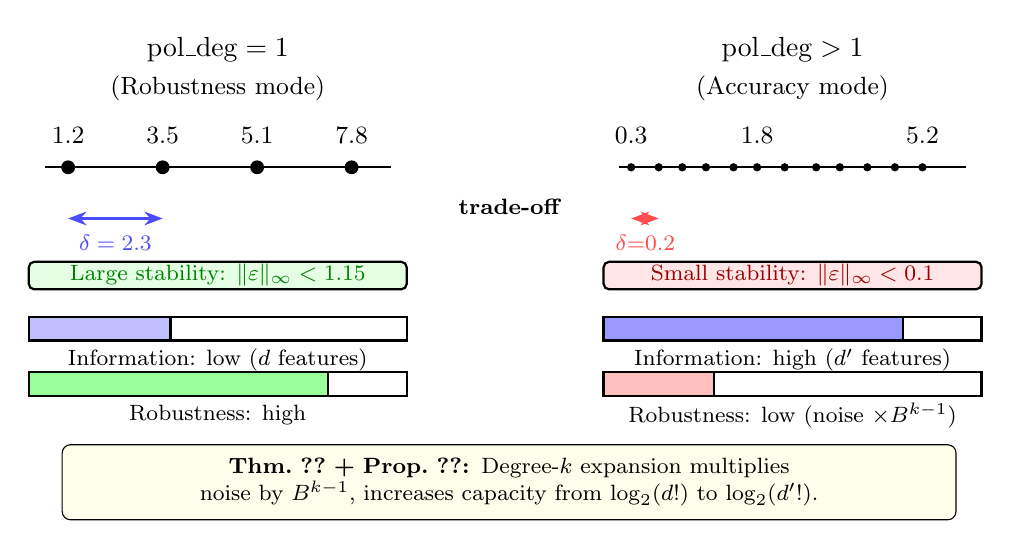
\begin{tikzpicture}[
    >=Stealth,
    lbl/.style={font=\small},
]
% === Left panel: degree 1 ===
\begin{scope}[shift={(0, 0)}]
\node[font=\normalsize\bfseries] at (2.2, 4.0) {$\mathrm{pol\_deg} = 1$};
\node[font=\small] at (2.2, 3.5) {(Robustness mode)};
% Number line
\draw[thick] (0, 2.5) -- (4.4, 2.5);
\foreach \x/\v in {0.3/1.2, 1.5/3.5, 2.7/5.1, 3.9/7.8} {
    \fill (\x, 2.5) circle (2.5pt);
    \node[lbl, above=5pt] at (\x, 2.5) {\v};
}
% Gap arrow
\draw[<->, thick, blue!70] (0.3, 1.85) -- (1.5, 1.85);
\node[lbl, blue!70, below=1pt, font=\footnotesize] at (0.9, 1.8) {$\delta = 2.3$};
% Stability box
\draw[thick, fill=green!10, rounded corners=2pt] (-0.2, 0.95) rectangle (4.6, 1.3);
\node[font=\footnotesize, green!50!black] at (2.2, 1.13) {Large stability: $\|\varepsilon\|_\infty < 1.15$};
% Information bar
\draw[thick, fill=blue!25] (-0.2, 0.3) rectangle (1.6, 0.6);
\draw[thick] (-0.2, 0.3) rectangle (4.6, 0.6);
\node[lbl, font=\footnotesize] at (2.2, 0.05) {Information: low ($d$ features)};
% Robustness bar
\draw[thick, fill=green!40] (-0.2, -0.4) rectangle (3.6, -0.1);
\draw[thick] (-0.2, -0.4) rectangle (4.6, -0.1);
\node[lbl, font=\footnotesize] at (2.2, -0.65) {Robustness: high};
\end{scope}
% === Central trade-off arrow ===
\draw[<->, ultra thick, black!50] (5.3, 2.0) -- (6.5, 2.0);
\node[font=\footnotesize\bfseries, fill=white, inner sep=3pt] at (5.9, 2.0) {trade-off};
% === Right panel: degree > 1 ===
\begin{scope}[shift={(7.3, 0)}]
\node[font=\normalsize\bfseries] at (2.2, 4.0) {$\mathrm{pol\_deg} > 1$};
\node[font=\small] at (2.2, 3.5) {(Accuracy mode)};
% Number line
\draw[thick] (0, 2.5) -- (4.4, 2.5);
\foreach \x in {0.15, 0.5, 0.8, 1.1, 1.45, 1.75, 2.1, 2.5, 2.8, 3.15, 3.5, 3.85} {
    \fill (\x, 2.5) circle (1.5pt);
}
\node[lbl, above=5pt] at (0.15, 2.5) {0.3};
\node[lbl, above=5pt] at (1.75, 2.5) {1.8};
\node[lbl, above=5pt] at (3.85, 2.5) {5.2};
% Gap arrow
\draw[<->, thick, red!70] (0.15, 1.85) -- (0.5, 1.85);
\node[lbl, red!70, below=1pt, font=\footnotesize] at (0.33, 1.8) {$\delta{=}0.2$};
% Stability box
\draw[thick, fill=red!10, rounded corners=2pt] (-0.2, 0.95) rectangle (4.6, 1.3);
\node[font=\footnotesize, red!60!black] at (2.2, 1.13) {Small stability: $\|\varepsilon\|_\infty < 0.1$};
% Information bar
\draw[thick, fill=blue!40] (-0.2, 0.3) rectangle (3.6, 0.6);
\draw[thick] (-0.2, 0.3) rectangle (4.6, 0.6);
\node[lbl, font=\footnotesize] at (2.2, 0.05) {Information: high ($d'$ features)};
% Robustness bar
\draw[thick, fill=red!25] (-0.2, -0.4) rectangle (1.2, -0.1);
\draw[thick] (-0.2, -0.4) rectangle (4.6, -0.1);
\node[lbl, font=\footnotesize] at (2.2, -0.65) {Robustness: low (noise $\times B^{k-1}$)};
\end{scope}
% === Bottom summary ===
\node[draw, rounded corners=3pt, fill=yellow!8, font=\footnotesize, text width=11cm, align=center, inner sep=5pt] at (5.9, -1.5) {
\textbf{Thm.~\ref{thm:stability} + Prop.~\ref{prop:poly-noise}:} Degree-$k$ expansion multiplies noise by $B^{k-1}$, increases capacity from $\log_2(d!)$ to $\log_2(d'!)$.
};
\end{tikzpicture}%
}
\caption{\textbf{The polynomial trade-off.} At degree 1 (left), features are well-separated: large gaps yield a wide stability region, but limited capacity. At degree $>1$ (right), cross-terms create small gaps: higher capacity but noise amplified by $B^{k-1}$, shrinking stability. This parameter is a master switch between robustness and accuracy.}
\label{fig:tradeoff}
\end{figure}


% ============================================================================
% 12. DISCUSSION
% ============================================================================
\section{Discussion}
\label{sec:discussion}

\subsection{What ArrowFlow Teaches Us}

The experiments tell a consistent story: ArrowFlow is competitive on clean accuracy, measurably superior in robustness scenarios (noise, privacy, missing data, batch effects), and limited by the information bottleneck of ordinal encoding. The deeper lesson is that competitive machine learning is possible without any floating-point parameters in the core computation. This is a proof of concept for a broader class of \emph{combinatorial learning systems} where the learned representation is a discrete structure (permutation, partition, matching) rather than a real-valued tensor. The existence proof matters: if permutation-based filters can compete with gradient-trained networks on standard benchmarks, what other combinatorial primitives---matchings, lattice orderings, graph homomorphisms---might serve as computational substrates for learning?

The architecture reveals a productive duality: the same properties that Arrow's theorem forbids in fair social choice (context dependence, dictatorship) are precisely what enable representational power in learning. This is not a coincidence---learning \emph{requires} breaking symmetry and introducing bias, and Arrow's axioms precisely characterize the symmetries that must be broken. The connection runs deeper than analogy: each ranking layer literally performs rank aggregation across filters, and the impossibility theorem explains why this aggregation cannot be simultaneously fair, context-free, and non-dictatorial. ArrowFlow's design exploits each violation as an inductive bias.

\subsection{Connections to Other Paradigms}

\paragraph{Self-Organizing Maps.}
Filter updates resemble Kohonen's competitive learning \citep{kohonen1990self}---the closest prototype moves toward the input. The key difference is that ArrowFlow prototypes are permutations and ``similarity'' is discrete edit distance. Both learn without gradients with winner-take-all dynamics. SOMs preserve topological relationships in a 2D grid; ArrowFlow preserves hierarchical composition via layer stacking.

\paragraph{Nearest-Neighbor Classification.}
The output sort layer performs 1-NN classification in permutation distance space. Hidden layers act as a learned nonlinear embedding into a space where class-conditional distances are more separable. The 2.5--12.5$\times$ improvement over kNN on the same encoded features (Table~\ref{tab:knn}) confirms that this embedding is genuinely useful---ArrowFlow does not merely store templates but learns discriminative ordinal representations.

\paragraph{Kernel Methods and the Mallows Kernel.}
The projection-plus-argsort encoding can be viewed as a random feature map for an implicit kernel on permutations, related to the Mallows model \citep{mallows1957nonnull}. The Mallows kernel $K(\pi, \sigma) = \exp(-\lambda \cdot d(\pi, \sigma))$ defines a probability distribution over permutations centered on a modal ranking, parameterized by a dispersion $\lambda$. ArrowFlow's filters can be seen as modal rankings, and the footrule distance plays the role of the Mallows dispersion. The multi-view ensemble then corresponds to a mixture of Mallows models, each defined by a different projection.

\paragraph{Rank Aggregation.}
Dwork et al.\ \citep{dwork2001rank} showed that combining ranked lists from multiple search engines via median-based methods on Kendall tau distance yields more robust rankings than any single source. ArrowFlow's multi-view ensemble implements a classification-oriented variant of the same principle: each view produces a ranked list of class distances, and majority vote aggregates these into a final prediction. The connection to Condorcet's jury theorem is direct---both systems improve through the wisdom of crowds.

\paragraph{Quantization and Discrete Representations.}
ArrowFlow's argsort encoding is an extreme form of quantization: from continuous features to ordinal positions. The broader quantization literature \citep{jacob2018quantization} shows that reduced-precision representations can improve robustness and computational efficiency. ArrowFlow pushes this idea to its logical endpoint---the representations are not merely low-precision but fundamentally \emph{combinatorial}. The polynomial degree trade-off discovered in Section~\ref{sec:tradeoff} may reflect a general principle: more aggressive discretization increases robustness but reduces information content.

\paragraph{The Forward-Forward Algorithm.}
Hinton's Forward-Forward algorithm \citep{hinton2022forward} replaces backpropagation with a local learning rule where each layer independently learns to distinguish ``positive'' from ``negative'' data. ArrowFlow's permutation-matrix accumulation shares this locality principle: each filter updates based on its own displacement evidence from the training signal, without requiring a global gradient computation. Both approaches demonstrate that alternatives to backpropagation can achieve competitive performance, though through very different mechanisms.

\subsection{Energy Analysis: The Case for Integer-Ordinal Hardware}
\label{sec:energy}

The preceding discussion frames ArrowFlow as an alternative computational paradigm. But \emph{why} would anyone prefer integer comparisons over floating-point multiply-accumulates? The answer is energy: ArrowFlow's core sort layers use \emph{no floating-point arithmetic}. Every operation---displacement computation, distance accumulation, filter updates, output ranking---is an integer comparison, subtraction, absolute value, or addition. This section quantifies the energy implications by comparing ArrowFlow's operation profile against a standard MLP on a per-layer and per-inference basis.

\paragraph{Operation counting.}
Consider a sort layer with $N$ filters over a vocabulary of size $V$. The forward pass for one data point performs:

\begin{enumerate}[leftmargin=2em]
  \item \textbf{Index table construction}: Build a lookup from input items to positions. With a pre-allocated index array, this is $V$ integer writes.
  \item \textbf{Displacement computation}: For each of $N$ filters, look up the input position of each of $V$ items (one integer table read), compute the signed displacement (one integer subtraction), take the absolute value, and add to a running sum. Total: $\sim 3NV$ integer operations.
  \item \textbf{Output ranking}: Argsort the $N$ distance values, requiring $O(N \log N)$ integer comparisons.
\end{enumerate}

The total is approximately $3NV + N\log_2 N$ integer operations per layer per data point. No multiply-accumulate (MAC) operations appear anywhere.

A comparable MLP layer ($V$ inputs, $N$ outputs) performs $NV$ floating-point MACs (each a multiply plus an add), $N$ bias additions, and $N$ activation evaluations: approximately $NV$ FP32 MACs total.

\paragraph{Energy per operation.}
Horowitz's widely cited ISSCC 2014 analysis \citep{horowitz2014energy} established the energy cost of arithmetic operations at 45nm CMOS, reproduced by Sze et al.\ \citep{sze2017efficient} in the context of DNN accelerator design:

\begin{table}[ht]
\centering
\caption{Energy per operation at 45nm CMOS \citep{horowitz2014energy}. ArrowFlow uses only operations in the top group; standard neural networks use operations in both groups.}
\label{tab:energy-ops}
\small
\begin{tabular}{lrl}
\toprule
Operation & Energy (pJ) & Used by \\
\midrule
8-bit integer ADD        & 0.03  & ArrowFlow \\
32-bit integer ADD/CMP   & 0.1   & ArrowFlow \\
32-bit integer MUL       & 3.1   & --- \\
\midrule
32-bit FP ADD            & 0.9   & MLP \\
32-bit FP MUL            & 3.7   & MLP \\
32-bit FP MAC            & 4.6   & MLP \\
\midrule
32-bit SRAM read (8KB)   & 5     & both \\
32-bit DRAM read         & 640   & both \\
\bottomrule
\end{tabular}
\end{table}

A single FP32 MAC costs 4.6\,pJ; a single integer comparison or addition costs 0.1\,pJ---a \textbf{46$\times$ gap} at the arithmetic level. If ArrowFlow's permutation indices fit in 8 bits ($V \leq 256$, which covers all configurations in this paper), the relevant integer operations cost 0.03\,pJ, widening the gap to \textbf{$\sim$150$\times$}.

\paragraph{Per-layer energy comparison.}
For a concrete comparison, consider ArrowFlow's \texttt{[128]} configuration on Digits ($V = 64$, $N = 128$) versus an MLP with a $64 \to 128$ hidden layer:

\begin{table}[ht]
\centering
\caption{Energy per layer, single data point. ArrowFlow \texttt{[128]} ($V{=}64$, $N{=}128$) vs.\ MLP ($64{\to}128$). All energies at 45nm CMOS.}
\label{tab:energy-layer}
\small
\begin{tabular}{lrrl}
\toprule
& Operations & Energy (pJ) & Op type \\
\midrule
\textbf{ArrowFlow sort layer} & & & \\
\quad Displacement (3NV) & 24,576  & 2,458 & INT32 @ 0.1\,pJ \\
\quad Argsort ($N\log_2 N$)& 896    & 90    & INT32 @ 0.1\,pJ \\
\quad \textit{Total} & 25,472  & \textbf{2,547} & \\
\midrule
\textbf{MLP layer} & & & \\
\quad Matrix multiply ($NV$ MACs) & 8,192 & 37,683 & FP32 @ 4.6\,pJ \\
\quad Bias + ReLU & 256 & 230 & FP32 \\
\quad \textit{Total} & 8,448 & \textbf{37,914} & \\
\midrule
\textbf{Ratio} & & \multicolumn{2}{l}{\textbf{14.9$\times$ in favor of ArrowFlow}} \\
\bottomrule
\end{tabular}
\end{table}

ArrowFlow performs $\sim$3$\times$ more operations but each costs $\sim$46$\times$ less energy, yielding a net \textbf{$\sim$15$\times$ arithmetic energy advantage} per layer.

\paragraph{Memory access energy.}
In practice, memory access dominates arithmetic cost in neural network inference \citep{sze2017efficient}. ArrowFlow's parameters are more compact: each filter is a permutation of $V$ items stored as 8-bit indices, requiring $NV$ bytes per layer. An MLP weight matrix requires $4NV$ bytes (FP32). For $N = 128$, $V = 64$:
\begin{itemize}[leftmargin=2em]
  \item ArrowFlow filter bank: $128 \times 64 = 8{,}192$ bytes (fits in 8KB SRAM)
  \item MLP weight matrix: $128 \times 64 \times 4 = 32{,}768$ bytes (requires 32KB)
\end{itemize}
When parameters fit in SRAM (5\,pJ per 32-bit read), the total memory energy for reading all weights once is 40,960\,pJ for the MLP vs.\ $\sim$10,240\,pJ for ArrowFlow's 8-bit indices---a 4$\times$ reduction. If parameters spill to DRAM (640\,pJ per read), the memory advantage becomes the dominant factor.

\paragraph{Full inference comparison.}
Table~\ref{tab:energy-full} compares full-inference energy for ArrowFlow's best Digits configuration (7-view ensemble, \texttt{[256]} layers, $V = 64$) against a single MLP ($64 \to 128 \to 10$):

\begin{table}[ht]
\centering
\caption{Full inference energy comparison on Digits. ArrowFlow: 7-view \texttt{[256]}, $V{=}64$. MLP: $64{\to}128{\to}10$. Arithmetic energy only (45nm CMOS).}
\label{tab:energy-full}
\small
\begin{tabular}{lrrr}
\toprule
Component & ArrowFlow (pJ) & MLP (pJ) \\
\midrule
Sort/hidden layer ($\times$7 views) & $7 \times 49{,}152 \times 0.1 = 34{,}406$ & $8{,}192 \times 4.6 = 37{,}683$ \\
Output layer ($\times$7 views) & $7 \times 768 \times 0.1 = 538$ & $1{,}280 \times 4.6 = 5{,}888$ \\
Majority vote & $\sim$70  & --- \\
\midrule
\textbf{Total arithmetic} & \textbf{35,014} & \textbf{43,571} \\
\textbf{Ratio} & \multicolumn{2}{c}{$1.2\times$ in favor of ArrowFlow} \\
\bottomrule
\end{tabular}
\end{table}

The 7-view ensemble erodes much of the per-operation advantage, reducing the ratio to $\sim$1.2$\times$ at the full-inference level. However, three factors make the real-world advantage substantially larger:
\begin{enumerate}[leftmargin=2em]
  \item \textbf{Memory bandwidth}: ArrowFlow's 8-bit parameters require 4$\times$ less memory bandwidth than FP32 weights. On memory-bound hardware (edge devices, neuromorphic chips), this translates directly to energy savings.
  \item \textbf{Parallelism}: The 7 views are embarrassingly parallel and operate on compact integer data, making them highly amenable to SIMD or multi-core execution with minimal inter-core communication.
  \item \textbf{No multiply hardware}: ArrowFlow requires only comparators, adders, and index tables---no floating-point multiply units. On an ASIC designed for ArrowFlow's operation profile, the die area and static power savings from eliminating FP multipliers would be substantial.
\end{enumerate}

\paragraph{Neuromorphic hardware alignment.}
ArrowFlow's computation maps naturally to neuromorphic architectures:

\begin{itemize}[leftmargin=2em]
  \item \textbf{Rank-order coding.} Thorpe's rank-order coding \citep{thorpe1998rapid, thorpe2001spike} encodes stimulus strength via the \emph{order} of neural spikes rather than firing rates---precisely the representation ArrowFlow operates on. A ranking filter in ArrowFlow corresponds to a stored spike-order template, and the footrule distance corresponds to the total spike-timing displacement. Imam and Cleland \citep{imam2020rapid} demonstrated that temporal-order-based classification on Intel Loihi achieves 1000$\times$ better energy efficiency than conventional CPU solutions.

  \item \textbf{Operation mapping.} ArrowFlow's displacement computation (integer subtraction + absolute value) maps to spike-timing difference circuits. The argsort operation maps to a sorting network---a fixed-topology circuit of compare-and-swap units. Batcher's bitonic sorting networks \citep{batcher1968sorting} require $O(N \log^2 N)$ comparators with a completely data-independent wiring pattern, ideal for fixed silicon. Each compare-and-swap costs ${\sim}0.15$\,pJ at 45nm, so sorting $N = 128$ distances requires ${\sim}100$\,pJ total---negligible compared to the displacement computation.

  \item \textbf{Event-driven sparsity.} Neuromorphic chips like Intel Loihi \citep{davies2018loihi} (23.6\,pJ/op at 14nm) and IBM TrueNorth \citep{merolla2014million} (26\,pJ/event at 28nm) achieve low energy through event-driven computation: neurons consume energy only when they spike. ArrowFlow's winner-take-all dynamics (Section~\ref{sec:arrow}, ND violation) create natural sparsity---most filters have large distances and only the closest few matter. An event-driven implementation could skip distance computation once a filter's partial distance exceeds the current minimum, reducing average-case energy well below the worst-case $3NV$ operations.
\end{itemize}

\paragraph{Summary.}
At the per-operation level, ArrowFlow's integer-only arithmetic is 15--150$\times$ more energy-efficient than FP32 MACs. The multi-view ensemble partially offsets this at the system level, but the combination of compact 8-bit parameters, zero floating-point hardware requirements, and natural alignment with neuromorphic spike-order coding makes ArrowFlow a compelling target for energy-constrained deployment. A custom ASIC or neuromorphic implementation of ArrowFlow's sort layers---comparators, integer adders, and index tables, with no multiply units---could achieve inference at a fraction of the energy cost of equivalently-accurate conventional networks.

\subsection{The Argsort Bottleneck: A Fundamental Limit}

The argsort encoding is simultaneously ArrowFlow's greatest strength and its most fundamental limitation. By converting real-valued features to orderings, ArrowFlow gains scale invariance, noise robustness (Theorem~\ref{thm:stability}), and privacy preservation---but loses all magnitude information. Theorem~\ref{thm:capacity} quantifies this: the ordinal representation has capacity $\log_2(d!) \approx d \log_2 d$ bits, finite and far below the infinite capacity of real-valued representations. Polynomial expansion increases $d$ and hence capacity, but Proposition~\ref{prop:poly-noise} shows this amplifies noise by a factor of $B^{k-1}$, weakening the stability bound. This tension---more information capacity vs.\ less noise robustness---is the formal basis of the polynomial trade-off documented in Section~\ref{sec:tradeoff}.

\subsection{Limitations}

\begin{itemize}[leftmargin=2em]
  \item \textbf{Computational cost:} Each forward pass is $O(NV)$ per data point. While the forward pass has been vectorized via batch distance computation, the backward pass remains sequential. This makes ArrowFlow approximately 10$\times$ slower than an equivalently-sized MLP per training iteration.
  \item \textbf{Information loss:} The argsort encoding discards magnitude information. Polynomial expansion mitigates but does not eliminate this, and introduces a robustness trade-off.
  \item \textbf{Scaling gap:} On larger datasets, ArrowFlow lags behind gradient-based methods. On MNIST (Section~\ref{sec:mnist-pca}), best ArrowFlow achieves 9.1\% vs.\ MLP's 4.2\%---a persistent $\sim$5pp gap. However, the gap narrows with wider architectures and has not plateaued, suggesting capacity rather than the learning principle is the bottleneck.
  \item \textbf{Natively ordinal data:} ArrowFlow's whole-permutation distance is too holistic when only local ordinal features are predictive (Sushi experiment, Section~\ref{sec:sushi}).
  \item \textbf{Rank-transform baseline:} On gene expression data (Section~\ref{sec:gene}), SVM on rank-transformed features achieves comparable or better batch-effect robustness than ArrowFlow native. The robustness advantage belongs to the ordinal representation principle, not to ArrowFlow specifically---though ArrowFlow provides this guarantee architecturally rather than as a preprocessing choice.
  \item \textbf{Hybrid architecture failure:} The tensor$\to$sort interface (Section~\ref{sec:hybrid}) destroys continuous representations via argsort discretization, preventing effective hybrid architectures.
  \item \textbf{Slow convergence:} The permutation-matrix accumulation makes conservative updates, requiring 200--500 iterations vs.\ $\sim$50 epochs for gradient-based methods.
\end{itemize}

\subsection{Future Directions}
\label{sec:future}

\begin{enumerate}[leftmargin=2em]
  \item \textbf{Batch vectorization:} The forward and backward passes process data points sequentially. Vectorizing via \texttt{scipy.cdist} or custom CUDA kernels could provide 10--50$\times$ speedup, making ArrowFlow practical for larger datasets.
  \item \textbf{Learned projections:} Replace random projection with end-to-end learned projections that minimize encoding loss while maintaining ensemble diversity. This could bridge the argsort bottleneck without abandoning the ordinal architecture.
  \item \textbf{Soft-sort encoding:} Using differentiable argsort approximations \citep{prillo2020softsort} to preserve partial magnitude information, potentially closing the gap on magnitude-sensitive datasets like Wine Quality.
  \item \textbf{Position-wise attention:} For natively ordinal data, a mechanism that weights individual item positions (rather than whole-permutation distances) could address the holistic-distance limitation exposed by the Sushi experiment.
  \item \textbf{Neuromorphic implementation:} ArrowFlow's integer-only arithmetic is 15--150$\times$ cheaper per operation than FP32 MACs (Section~\ref{sec:energy}). A custom ASIC implementing sort layers as comparator arrays and index tables could make inference dramatically cheaper than conventional networks, particularly on neuromorphic platforms \citep{davies2018loihi, merolla2014million} where spike-order coding is native.
  \item \textbf{Mode selection framework:} The polynomial trade-off (Section~\ref{sec:tradeoff}) suggests a practical deployment strategy: automatically select $\mathrm{pol\_deg}$=1 when the data is noisy, privacy-constrained, or incomplete; $\mathrm{pol\_deg}>1$ when clean accuracy is paramount.
  \item \textbf{Text and sequence domains:} The CountVectorizer nonzero encoding (converting word presence to native permutations) opens a path for applying ArrowFlow to text classification without the projection pipeline. Initial IMDB experiments are underway.
  \item \textbf{Broader combinatorial primitives:} Displacement-accumulation generalizes beyond permutations to other discrete structures---matchings, partial orders, lattice elements---potentially yielding a family of combinatorial learning architectures.
\end{enumerate}


% ============================================================================
% 12. CONCLUSION
% ============================================================================
\section{Conclusion}
\label{sec:conclusion}

ArrowFlow demonstrates that machine learning can operate effectively in the space of permutations. The architecture processes information through ranking filters---discrete permutations learned via motion accumulation rather than gradient descent---and achieves competitive classification accuracy through multi-view ensembles of diverse ordinal projections.

The key empirical findings, across 7 UCI datasets, MNIST, gene expression cancer classification, and preference data, with GridSearchCV-tuned baselines, are:
\begin{enumerate}[leftmargin=2em]
  \item ArrowFlow \textbf{beats all baselines on Iris} (2.7\% vs.\ 3.3\%) and is competitive on 5 of 7 UCI datasets, proving that zero-floating-point-parameter architectures can match gradient-trained networks.
  \item The \textbf{polynomial degree acts as a master switch} between accuracy and robustness. At degree~1, ArrowFlow provides measurable noise robustness (8--28\% less degradation), near-zero-cost privacy preservation (+0.5pp under rank transforms), and superior missing-feature handling (beats all baselines on Iris at 50\% masking). At higher degrees, clean accuracy improves but perturbation amplification erases these advantages.
  \item On gene expression data, ordinal encoding provides \textbf{perfect invariance to monotone batch effects}: SVM on raw values collapses from 0.6\% to 82.6\% under $\log$, $\sqrt{}$, or global scaling, while rank-based methods remain stable at 2.5\%. Under realistic per-gene batch effects ($\sigma \leq 0.5$), rank methods are unaffected while raw-input SVM error increases $28\times$. ArrowFlow embodies this ordinal robustness architecturally.
  \item On \textbf{MNIST via PCA}, ArrowFlow achieves 9.1\% error using only ordinal comparisons. It \textbf{scales strongly} with width and depth (18.7\%$\to$9.1\%), and the scaling curve has not plateaued, suggesting capacity is the bottleneck.
  \item The \textbf{multi-view ensemble} with diverse projections is the single most impactful component, reducing error by 2--3$\times$.
  \item \textbf{Freezing the output layer} consistently improves performance, a novel training strategy analogous to fixing classifier heads in transfer learning.
  \item ArrowFlow's \textbf{learning genuinely helps}: 2.5--12.5$\times$ improvement over kNN on the same encoded features proves that filter updates learn discriminative ordinal structure.
\end{enumerate}

Beyond empirics, the theoretical analysis (Section~\ref{sec:theory}) provides formal grounding: the argsort stability theorem (Theorem~\ref{thm:stability}) and its Gaussian corollary explain the noise robustness; the information capacity theorem (Theorem~\ref{thm:capacity}) quantifies the encoding bottleneck at $\log_2(d!)$ bits; the polynomial noise amplification result (Proposition~\ref{prop:poly-noise}) explains the accuracy--robustness trade-off; and the accumulation consistency result (Proposition~\ref{prop:convergence}) guarantees that the learning rule converges to the optimal filter ordering.

The deeper contribution is conceptual: ArrowFlow shows that the violations of Arrow's social-choice axioms---context dependence, specialization, symmetry breaking---are not obstacles but \emph{mechanisms} for learning. Each ranking layer is a micro-democracy of filters whose deliberate ``unfairness'' creates nonlinearity, sparsity, and hierarchical composition. This reframes neural computation through the lens of combinatorics and voting theory, opening a new research direction at the intersection of social choice, rank-order coding, and representation learning.

ArrowFlow is not the final word in ordinal machine learning---it is the first. The encoding bottleneck, the scaling gap, and the holistic-distance limitation are real constraints that bound the current system's practical applicability. But the fact that a system with \emph{zero floating-point parameters} in its core layers can achieve 2.7\% error on Iris, 9.1\% on MNIST, and perfect batch-effect invariance on gene expression data---and that we can \emph{prove} why its robustness properties hold---is, we believe, a foundation worth building on.


% ============================================================================
% REFERENCES
% ============================================================================
\bibliographystyle{plainnat}
\bibliography{references_arrowflow}


\end{document}
